%! TeX program = lualatex
\documentclass{tesis}
\usepackage{fontspec}
\usepackage{mdwtab}
\usepackage{lscape}




\setmainfont{Times New Roman}

\newcommand{\autor}{Tigselema Pacheco Alex Ignacio}
\newcommand{\cedulaAutor}{1803834371}
\newcommand{\tutor}{Leonardo David Torres Valverde}
\newcommand{\lugarFechaPrelims}{Ambato, julio 2024}
\newcommand{\tema}{Sistema web y móvil para la sistematización de la gestión administrativa y de asambleas del conjunto habitacional {\textquotedblleft}El Portal de la Viña{\textquotedblright}}
\newcommand{\elaboradopor}{Elaborado por: el investigador}


\begin{document}

%Start counting pages from 2 in roman numbers
\pagenumbering{roman}

%A. Paginas preliminares
\addcontentsline{toc}{chapter}{\bfseries \uppercase{PORTADA}}
\begin{titlepage}
	\begin{center}

		
\includegraphics[width=50mm]{resources/images/logo-uta.png}

		\textbf{\uppercase{
				Universidad Técnica de Ambato \\
				\vspace{5mm}
				Facultad de Ingeniería en sistemas, electrónica e industrial \\
				\vspace{5mm}
				carrera de software \\
			}}

		\vspace{5mm}
		\textbf{Tema:}
		\vspace{5mm}

		\begin{tabular}[c]{>{\centering\arraybackslash}p{0.97\textwidth}}
			\toprule
			{\bfseries\MakeUppercase\tema} \\
			\bottomrule
		\end{tabular}

    \vspace{24pt}
		Trabajo de titulación modalidad Proyecto de investigación, presentado
		previo a la obtención del título de Ingeniero de Software

		\vspace{5mm}
		\textbf{\uppercase{área:}} Software\\
		\vspace{5mm}
		\textbf{\uppercase{línea de investigacion:}} Desarrollo de Software\\
		\vspace{5mm}
		\textbf{\uppercase{autor:}} \autor \\
		\vspace{5mm}
		\textbf{\uppercase{tutor:}} Ing. \tutor, Mg.\\

		\vfill
		Ambato - Ecuador\\
		julio - 2024

	\end{center}
\end{titlepage}


\setcounter{page}{2}
%TODO
\chapter*{aprobación del tutor}
\addcontentsline{toc}{chapter}{\bfseries \uppercase{aprobación del tutor}}

En calidad de tutor del trabajo de titulación con el tema:
{\MakeUppercase\tema},
desarrollado bajo
la modalidad Proyecto de Investigación, por el señor \autor,
estudiante de la Carrera de Software, de la Facultad de Ingeniería en Sistemas, Electrónica e Industrial, de la
Universidad Técnica de Ambato, me permito indicar que el estudiante ha sido tutorado
durante todo el desarrollo del trabajo hasta su conclusión, de acuerdo a lo dispuesto en
el Artículo 17 del Reglamento para la Titulación de Grado en la Universidad Técnica
de Ambato y el numeral 6.3 del instructivo del reglamento referido.
\\
\\
\begin{flushright}
	\lugarFechaPrelims.
\end{flushright}

\vspace*{5cm}
\begin{center}
	\begin{tabular}{c}
		\hbox to 7cm{\leaders\hbox to 5pt{\hss - \hss}\hfil} \\
		Ing. \tutor, Mg.\\
		TUTOR
	\end{tabular}
\end{center}

%TODO
\chapter*{autoría}
\addcontentsline{toc}{chapter}{\bfseries \uppercase{autoría}}
El presente trabajo de titulaci\'on con el tema: {\MakeUppercase\tema} es absolutamente original, auténtico y personal y ha observado
los preceptos establecidos en la Disposición General Quinta del Reglamento para la
Titulación de Grado en la Universidad Técnica de Ambato. En tal virtud, el contenido,
efectos legales y académicos que se desprenden del mismo son de exclusiva
responsabilidad del autor.
\\
\\
\\
\begin{flushright}
	\lugarFechaPrelims.
\end{flushright}

\vspace*{5cm}
\begin{center}
	\begin{tabular}{c}
		\hbox to 7cm{\leaders\hbox to 5pt{\hss - \hss}\hfil} \\
		Alex Ignacio Tigselema Pacheco                      \\
		C.C. 1803834371                                      \\
		AUTOR
	\end{tabular}
\end{center}

%TODO
\chapter*{derechos de autor}
\addcontentsline{toc}{chapter}{\bfseries \uppercase{derechos de autor}}
Autorizo a la Universidad Técnica de Ambato para que reproduzca total o parcialmente
este trabajo de titulación dentro de las regulaciones legales e institucionales
correspondientes. Además, cedo todos mis derechos de autor a favor de la institución
con el propósito de su difusión pública, por lo tanto, autorizo su publicación en el
repositorio virtual institucional como un documento disponible para la lectura y uso
con fines académicos e investigativos de acuerdo con la Disposición General Cuarta
del Reglamento para la Titulación de Grado en la Universidad Técnica de Ambato.
\begin{flushright}
	\lugarFechaPrelims.
\end{flushright}

\vspace*{5cm}
\begin{center}
	\begin{tabular}{c}
		\hbox to 7cm{\leaders\hbox to 5pt{\hss - \hss}\hfil} \\
		Alex Ignacio Tigselema Pacheco                      \\
		C.C. 1803834371                                      \\
		AUTOR
	\end{tabular}
\end{center}

%TODO
\chapter*{aprobación del tribunal de grado}
\addcontentsline{toc}{chapter}{\bfseries \uppercase{aprobación del tribunal de grado}}
En calidad de par calificador del informe final del trabajo de titulación presentado por el señor \autor, estudiante de la Carrera de Software,
de la Facultad de Ingeniería en Sistemas,
Electrónica e Industrial, bajo la Modalidad Proyecto de Investigación, titulado
	{\MakeUppercase\tema}
nos permitimos informar que el trabajo ha sido revisado
y calificado de acuerdo al Artículo 19 del Reglamento para la Titulación de Grado en
la Universidad Técnica de Ambato y el numeral 6.4 del instructivo del reglamento
referido. Para cuya constancia suscribimos, conjuntamente con la señora Presidente
del Tribunal.
\begin{flushright}
	\lugarFechaPrelims.
\end{flushright}


\vspace*{4cm}
\begin{center}
	\begin{tabular}{c}
		\hbox to 7cm{\leaders\hbox to 5pt{\hss - \hss}\hfil} \\
		Ing. Elsa Pilar Urrutia Urrutia, Mg.                 \\
		PRESIDENTE DEL TRIBUNAL                              \\
	\end{tabular}
\end{center}
\vspace*{20mm}
\begin{center}
	\begin{tabular}{c c}
		\hbox to 7cm{\leaders\hbox to 5pt{\hss - \hss}\hfil} & \hbox to 7cm{\leaders\hbox to 5pt{\hss - \hss}\hfil} \\
		xxxxxxxxxxxxxxxxxxx               & xxxxxxxxxxxxxxxxxxxxxx             \\
		PROFESOR CALIFICADOR                                 & PROFESOR CALIFICADOR
	\end{tabular}
\end{center}

\newpage
\vspace*{\fill}
\begin{flushright}
  \footnotesize
	\begin{minipage}{0.5\textwidth}
		\begin{flushright}
      \phantomsection
			\uppercase{\textbf{Dedicatoria}}
		\end{flushright}
		\itshape

		\bigbreak
		\begin{flushright}
			\textbf{Alex Ignacio Tigselema Pacheco}
		\end{flushright}
	\end{minipage}
\end{flushright}
\vspace*{\fill}
\addcontentsline{toc}{chapter}{\bfseries DEDICATORIA}

\newpage
\vspace*{\fill}
\begin{flushright}
	\footnotesize
	\begin{minipage}{0.5\textwidth}
		\begin{flushright}
			\phantomsection
			\uppercase{\textbf{Agradecimientos}}
		\end{flushright}
		\itshape


		\bigbreak
		\begin{flushright}
			\textbf{Alex Ignacio Tigselema Pacheco}
		\end{flushright}
	\end{minipage}
\end{flushright}
\vspace*{\fill}
\addcontentsline{toc}{chapter}{\bfseries AGRADECIMIENTO}

\chapter*{Anexos}
\addcontentsline{toc}{chapter}{\bfseries\uppercase{Anexos}}

% \addtocontents{toc}{\protect\setcounter{tocdepth}{0}}
\appendix

\renewcommand{\thetable}{\theappendixs\arabic{table}}
\renewcommand{\thefigure}{\theappendixs\arabic{figure}}
\renewcommand{\thelstlisting}{\theappendixs\arabic{lstlisting}}
\captionsetup{list=no}

\appendixs{Guía de entrevista a la directiva del conjunto habitacional {\textquotedblleft}El Portal de la Viña{\textquotedblright}}
\label{app:guia-entrevista-directiva}
\begin{table}[H]
	\caption{Guía de entrevista a la directiva del conjunto habitacional {\textquotedblleft}El Portal de la Viña{\textquotedblright}}
	\label{tab:guia-entrevista-directiva}


	\begin{center}
		\begin{footnotesize}
		\begin{tabular}[c]{|p {0.03\textwidth}|p{0.6\textwidth}|p{0.15\textwidth}|p{0.15\textwidth}|}
			\hline
			\multicolumn{1}{|c|}{\textbf{N.}} & \multicolumn{1}{c|}{\textbf{Pregunta}} & \multicolumn{1}{c|}{\textbf{Respuesta}} & \multicolumn{1}{c|}{\textbf{Observación}} \\
			\hline
			1 & ¿Cuáles son sus funciones administrativas o financieras como parte de la directiva? & & \\ \hline
			2 & ¿Cómo miembro de la directiva tiene alguna función extra que la realice de forma extraordinaria como parte de su iniciativa? & &\\ \hline
			3 & ¿Qué reportes, documentos o certificados entrega como parte de directiva y con qué información? & &\\ \hline
			4 & ¿Cuál es el proceso actual para la adquisición de un parqueadero tanto particular como de zona azul y en el caso de requerir alguna información o documento, existe la posibilidad de poder entregar alguno de manera digital? & &\\ \hline
			5 & ¿De que manera se lleva el registro de los parqueaderos? & &\\ \hline
			6 & ¿Cuáles es el proceso actual para la adquisición de servicios de proveedores (guardianía, internet, jardinería, etc.)? & &\\ \hline
			7 & ¿De qué manera se lleva la contabilidad del conjunto habitacional y que reportes se suelen presentar y con qué información? & &\\ \hline
			8 & ¿De que manera se comunica a los residentes del condominio eventos sociales o convocatorias de asambleas? & &\\ \hline
			9 & ¿Cuál es el proceso actual para el registro de asistencia y las votaciones en las asambleas? & &\\ \hline
			10 & ¿Cuándo una residente falta a una reunión de asamblea que penalizaciones o multas recibe? & &\\ \hline
			11 & ¿Qué problemas o inconvenientes han tenido con los procesos administrativos o financieros actuales? & &\\ \hline
			12 & ¿Actualmente cómo funciona el buzón de quejas/sugerencias? & &\\ \hline
			13 & ¿Dónde manejan la información de los pagos (multas, alícuotas, parqueaderos, etc.), asambleas, eventos sociales, pagos a proveedores y demás información importante? & &\\
			\hline
		\end{tabular}
		\end{footnotesize}
	\end{center}

\end{table}

\newpage
\appendixs{Encuesta de necesidades a los residentes del conjunto habitacional {\textquotedblleft}El Portal de la Viña{\textquotedblright}}
\label{app:encuesta-residentes}

\begin{center}
	\begin{small}
		\begin{longtable}[c]{|p{0.6\textwidth}|p{0.35\textwidth}|}
			\caption{Encuesta de necesidades a los residentes del conjunto habitacional {\textquotedblleft}El Portal de la Viña{\textquotedblright}} \\
			\hline
			\textbf{Pregunta} & \textbf{Respuesta} \\
			\hline
			¿Cree usted que el proceso actual para obtener la información de las obligaciones financieras (pagos, multas, etc.) de su domicilio es eficiente? &
			\begin{itemize}
				\item Totalmente de acuerdo
				\item De acuerdo
				\item Ni de acuerdo ni en desacuerdo
				\item En desacuerdo
				\item Totalmente en desacuerdo
			\end{itemize} \\
			\hline
			¿Con que frecuencia solicita la información de las obligaciones financieras (pagos, multas, etc.) de su domicilio a tesorería? &
			\begin{itemize}
				\item Por lo menos una vez al mes
				\item Dos veces al mes
				\item Tres veces al mes
				\item Cuatro veces al mes
				\item Más de cuatro veces al mes
			\end{itemize}\\
			\hline
			¿Cree usted que el proceso actual para el registro de asistencias durante la asamblea es eficiente en términos de tiempo? &
			\begin{itemize}
				\item Totalmente de acuerdo
				\item De acuerdo
				\item Ni de acuerdo ni en desacuerdo
				\item En desacuerdo
				\item Totalmente en desacuerdo
			\end{itemize} \\
			\hline
			¿Considera usted que el conteo actual de las votaciones durante las asambleas es transparente y eficiente? &
			\begin{itemize}
				\item Totalmente de acuerdo
				\item De acuerdo
				\item Ni de acuerdo ni en desacuerdo
				\item En desacuerdo
				\item Totalmente en desacuerdo
			\end{itemize} \\
			\hline
			¿Ha experimentado retrasos en la entrega de los comprobantes de pagos? &
			\begin{itemize}
				\item Si
				\item No
			\end{itemize} \\
			\hline
			¿Con que frecuencia olvida que el pago de alícuotas de su domicilio esta por vencer? &
			\begin{itemize}
				\item Muy frecuentemente
				\item Frecuentemente
				\item Ocasionalmente
				\item Raramente
				\item Nunca
			\end{itemize}\\
			\hline
			¿Con que frecuencia ha utilizado el buzón de quejas/sugerencias? &
			\begin{itemize}
				\item Nunca lo he usado
				\item Al menos una vez al mes
				\item Dos veces al mes
				\item Tres veces al mes
				\item Más de tres veces al mes
			\end{itemize} \\
			\hline
			¿Considera usted que los medios actuales (whatsapp/pizarrón en la garita) que utiliza la directiva para publicar comunicados son eficientes? &
			\begin{itemize}
				\item Totalmente de acuerdo
				\item De acuerdo
				\item Ni de acuerdo ni en desacuerdo
				\item En desacuerdo
				\item Totalmente en desacuerdo
			\end{itemize} \\
			\hline
			¿Preferiría utilizar una aplicación móvil que le permita revisar la información de las obligaciones financieras de su domicilio, el registro de su asistencia y voto durante las asambleas, se le envíen notificaciones recordándole los pagos por vencer o que ha sido multado por alguna infracción? &
			\begin{itemize}
				\item Si
				\item No
			\end{itemize} \\
			\hline
		\end{longtable}
	\end{small}
\end{center}

\newcolumntype{C}[1]{>{\centering\arraybackslash}m{#1}}
\appendixs{Encuesta TAM del sistema web administrativo}
\label{app:encuesta-tam}
\begin{center}
	\begin{small}
		\begin{table}[ht]
		\begin{center}
			\caption{Encuesta de aceptación TAM \#1}
			\bigbreak
			\begin{tabular}{ *{5}{C{2cm}} }
				\hline
				\multicolumn{5}{ c }{\textbf{ENCUESTA DE ACEPTACIÓN TAM SISTEMA WEB}} \\ \hline
				\multicolumn{5}{p{.7\textwidth}}{En una escala de Likert indique su grado de aceptación con las siguientes ponderaciones: } \\ \hline
				\centering 1             & 2             & 3       & 4          & 5                     \\ \hline
				Totalmente en desacuerdo & En desacuerdo & Neutral & De acuerdo & Totalmente de acuerdo \\ \hline
				\textbf{PU} & \multicolumn{4} {c}{\textbf{Utilidad Percibida}} \\ \hline
				PU1 & \multicolumn{4}{p{.7\textwidth}}{El sistema facilita las tareas de gestión del conjunto residencial} \\ \hline
				PU2 & \multicolumn{4}{p{.7\textwidth}}{Mejora la eficiencia en las operaciones diarias del conjunto residencial} \\ \hline
				PU3 & \multicolumn{4}{p{.7\textwidth}}{Proporciona información relevante para la toma de decisiones} \\ \hline
				PU4 & \multicolumn{4}{p{.7\textwidth}}{Mejora la calidad de vida/comodidad para los residentes} \\ \hline
				\textbf{PEOU} & \multicolumn{4}{ c }{\textbf{Facilidad de Uso Percibida}} \\ \hline
				PEOU1 & \multicolumn{4}{p{.7\textwidth}}{Es fácil aprender a utilizar el sistema de gestión residencial} \\ \hline
				PEOU2 & \multicolumn{4}{p{.7\textwidth}}{La navegación por el sistema es clara y lógica} \\ \hline
				PEOU3 & \multicolumn{4}{p{.7\textwidth}}{El diseño de la interfaz es intuitivo y amigable} \\ \hline
				PEOU4 & \multicolumn{4}{p{.7\textwidth}}{Es cómodo interactuar desde diferentes navegadores web} \\ \hline
			\end{tabular}
			\label{tab:tam_encuesta_web}
			\bigbreak
		\end{center}
	\end{table}
	\end{small}
\end{center}

\newpage
\newcolumntype{C}[1]{>{\centering\arraybackslash}m{#1}}
\appendixs{Encuesta TAM del sistema web administrativo}
\label{app:encuesta-tam-app}
\begin{center}
	\begin{small}
		\begin{table}[h]
			\begin{center}
				\caption{Encuesta de aceptación TAM \#2}
				\begin{tabular}{ *{5}{C{2cm}} }
					\hline
					\multicolumn{5}{ c }{\textbf{ENCUESTA DE ACEPTACIÓN TAM APLICACIÓN MÓVIL}} \\ \hline
					\multicolumn{5}{p{.7\textwidth}}{En una escala de Likert indique su grado de aceptación con las siguientes ponderaciones: } \\ \hline
					\centering 1             & 2             & 3       & 4          & 5                     \\ \hline
					Totalmente en desacuerdo & En desacuerdo & Neutral & De acuerdo & Totalmente de acuerdo \\ \hline
					\textbf{PU} & \multicolumn{4} {c}{\textbf{Utilidad Percibida}} \\ \hline
					PU1 & \multicolumn{4}{p{.7\textwidth}}{La aplicación ofrece información relevante sobre próximos eventos en el conjunto residencial} \\ \hline
					PU2 & \multicolumn{4}{p{.7\textwidth}}{Las notificaciones de pagos son claras y fáciles de comprender en la aplicación.} \\ \hline
					PU3 & \multicolumn{4}{p{.7\textwidth}}{La opción de votaciones dentro de la aplicación es útil y accesible.} \\ \hline
					PU4 & \multicolumn{4}{p{.7\textwidth}}{La aplicación mejora la interacción y la comunicación entre los residentes.} \\ \hline

					\textbf{PEOU} & \multicolumn{4}{ c }{\textbf{Facilidad de Uso Percibida}} \\ \hline
					PEOU1 & \multicolumn{4}{p{.7\textwidth}}{Es sencillo navegar por la aplicación para encontrar la información deseada.} \\ \hline
					PEOU2 & \multicolumn{4}{p{.7\textwidth}}{El diseño de la aplicación es intuitivo y fácil de comprender.} \\ \hline
					PEOU3 & \multicolumn{4}{p{.7\textwidth}}{La aplicación ofrece una experiencia cómoda al interactuar desde distintos dispositivos móviles.} \\ \hline
					PEOU4 & \multicolumn{4}{p{.7\textwidth}}{La función de votación en la aplicación es fácil de usar y comprender.} \\ \hline
				\end{tabular}
				\label{tab:tam_encuesta_app}
				\bigbreak
				Elaborado por: el investigador
			\end{center}
		\end{table}
	\end{small}
\end{center}

\newpage
\appendixs{Dependencias de la API} \label{app:dependencias-api}

\begin{figure}[H]
    \centering
    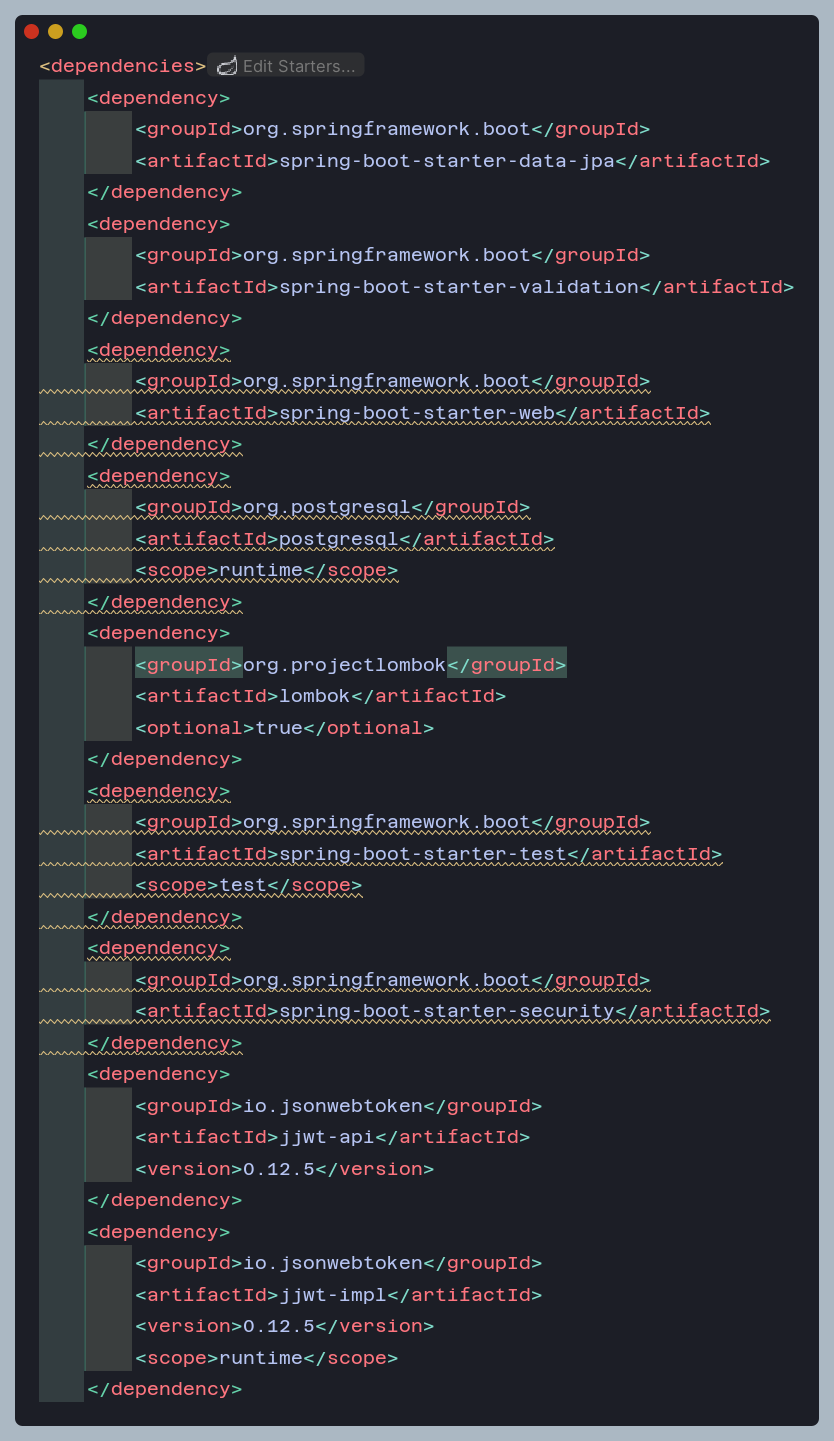
\includegraphics[width=.8\textwidth]{resources/images/dependencias-anexo-1}\label{fig:dependencias Api 1}
\end{figure}

\begin{figure}[H]
    \centering
    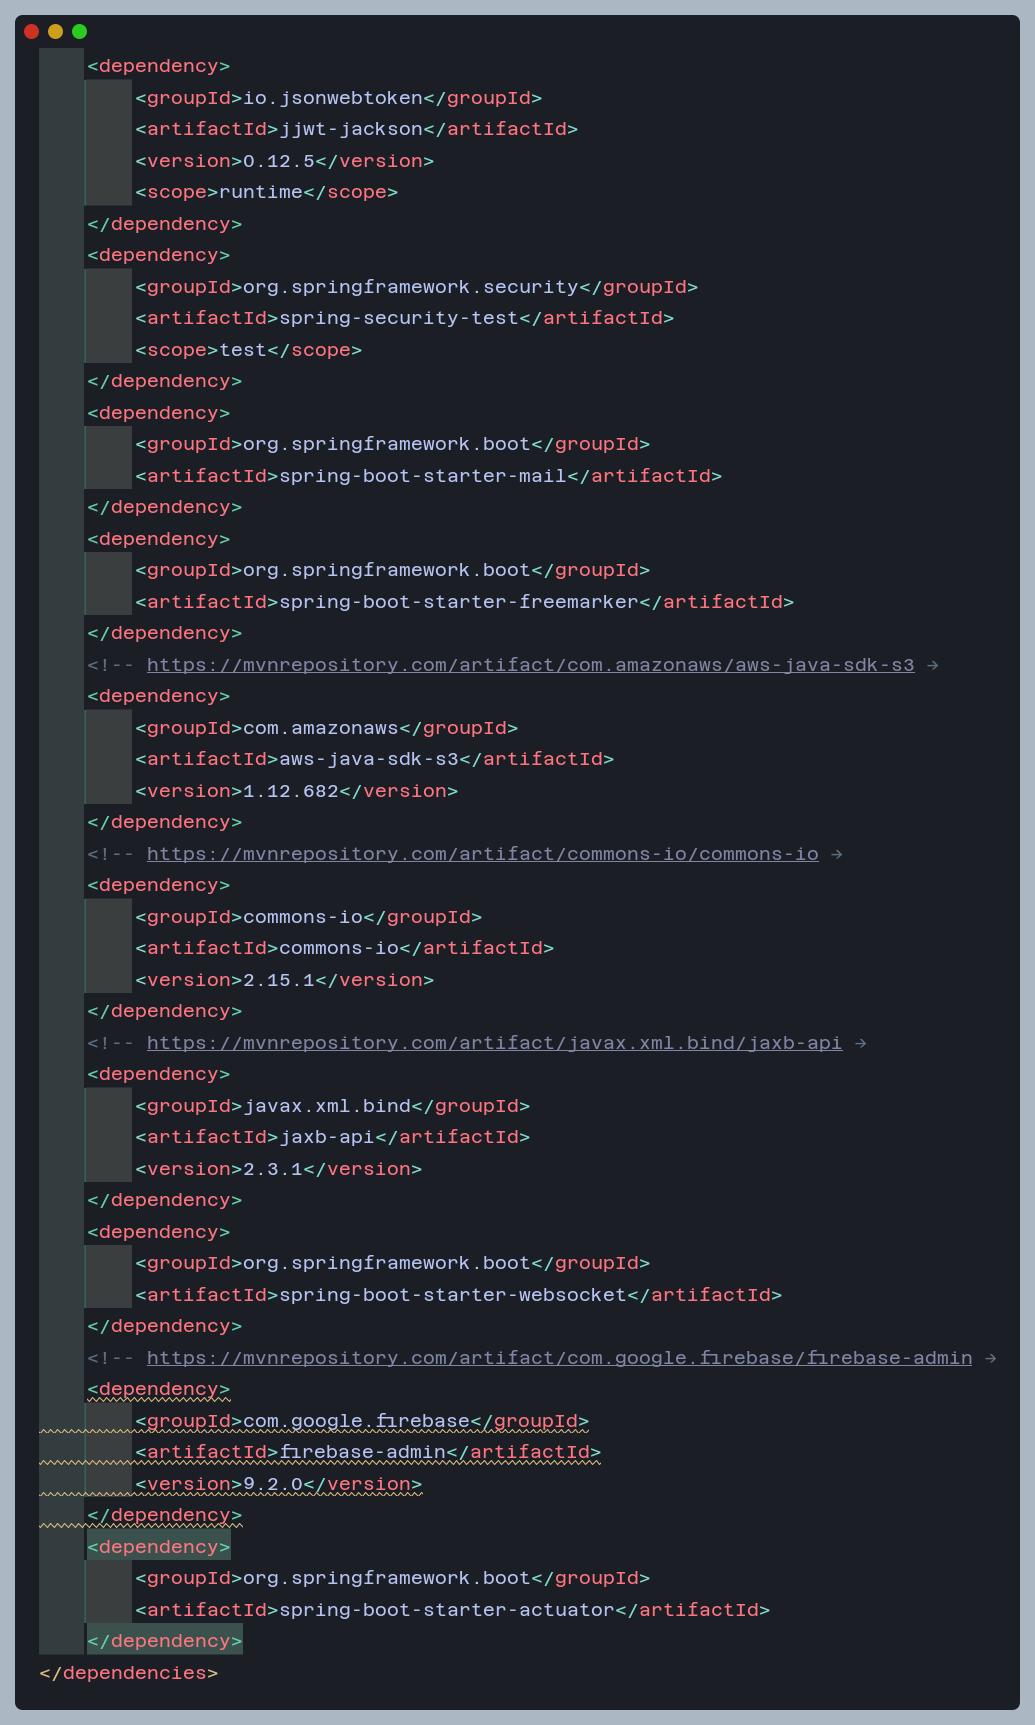
\includegraphics[width=.8\textwidth]{resources/images/dependencias-anexo-2}\label{fig:dependencias Api 2}
\end{figure}


\chapter*{resumen ejecutivo}

El conjunto habitacional {\textquotedblleft}El Portal de la Viña{\textquotedblright} consta de 303 residencias, lo cual dificulta el control de los procesos administrativos por parte de la directiva, dando lugar a desafíos en la gestión de los parqueaderos, convocatorias y en tesorería, ya que estos procesos se realizan de manera manual.
\bigbreak
El presente proyecto implementa un sistema de gestión web junto con una aplicación móvil para sistematizar los procesos administrativos y financieros del conjunto habitacional. Además, se utiliza la geolocalización como mecanismo de verificación de la asistencia y las votaciones en las asambleas. Para ello, se emplea la fórmula de Haversine para calcular con precisión la distancia entre la ubicación del residente y el punto de la asamblea, asegurando así que solo los asistentes presentes puedan participar en las votaciones.
\bigbreak
El sistema de gestión del conjunto habitacional incluye módulos para la administración de propietarios, residencias, pagos, convocatorias, guardianía y parqueaderos. Se emplearon tecnologías modernas como los frameworks Angular e Ionic para el cliente web y móvil, respectivamente. Para el desarrollo de la interfaz de programación de aplicaciones (API), se utilizó el framework Spring Boot junto con PostgreSQL como gestor de base de datos.
\bigbreak
La validación del sistema implementado se realizó aplicando el modelo de aceptación de tecnología (TAM) a los residentes del conjunto habitacional, teniendo como resultado una aceptación positiva del sistema propuesto. Se espera que la implementación de este sistema mejore la eficiencia y la transparencia en la administración del conjunto habitacional.

\vfill
\textbf{Palabras clave:} Sistematización, conjunto habitacional, Framework, geolocalización, Angular, Ionic, Spring boot.

\newpage
\chapter*{abstract}
\addcontentsline{toc}{chapter}{\bfseries \uppercase{ABSTRACT}}

The {\textquotedblleft}El Portal de la Viña{\textquotedblright} housing complex consists of 303 residences, which makes it difficult for the board of directors to control the administrative processes, giving rise to challenges in the management of parking spaces, calls, and in treasury, since these processes are carried out manually.
\bigbreak
This project implements a web management system along with a mobile application to systematize the administrative and financial processes of the housing complex. In addition, geolocation is used as a mechanism to verify attendance and voting at assemblies. To do this, the Haversine formula is used to accurately calculate the distance between the resident's location and the assembly point, thus ensuring that only those present can participate in the votes.
\bigbreak
The housing complex management system includes modules for the administration of owners, residences, payments, calls, guardianship, and parking. Modern technologies such as Angular and Ionic frameworks were used for the web and mobile client, respectively. For the development of the application programming interface (API), the Spring Boot framework was used along with PostgreSQL as a database manager.
\bigbreak
The validation of the implemented system was carried out by applying the technology acceptance model (TAM) to the residents of the housing complex, resulting in a positive acceptance of the proposed system. The implementation of this system is expected to improve efficiency and transparency in the administration of the housing complex.

\vfill
\textbf{Keywords:} Systematization, Housing complex, Framework, Geolocation, Angular, Ionic, Spring boot.



%B. Contenidos
%Change counting to arabic numbers
\newpage
\renewcommand{\thepage}{\arabic{page}}% Roman page numbers
\setcounter{page}{1}
\chapter{MARCO TEÓRICO}\label{ch:marco-teorico}
\section{Tema de investigación}\label{sec:tema-de-investigacion}
\uppercase{\MakeUppercase\tema}
\subsection{Planteamiento del problema}\label{subsec:planteamiento-del-problema}
En\cite{MoranSalazar} el autor menciona que los avances tecnológicos han sido muy relevantes en la sociedad actual, debido a que han permitido la optimización de procesos y la automatización de tareas, lo cual ha facilitado a las empresas y organizaciones ser más eficientes y productivas.
En el caso administrativo, las herramientas tecnológicas ofrecen soluciones automatizadas mediante sistemas computacionales que reemplazan a los sistemas manuales tradicionales.
\bigbreak
En\cite{INEC}, menciona que Ambato según el censo del 2022 realizado por el Instituto Nacional de Estadística y Censos(INEC) se ha registrado un total de 153948 viviendas particulares y 234 viviendas colectivas con un promedio de 3.18 habitantes por vivienda.
En estos casos, según\cite{Propiedad_Horizontal} en su Artículo 11 de la Ley de Propiedad horizontal los copropietarios tienen derecho a establecer sus propias normativas y reglamentos internos con la finalidad de poder crear modelos de gestión internos.
En este sentido la gestión de los condóminios o departamentos se realizan mediante sistemas manuales lo cual al ser conjuntos residenciales son muy ineficientes debido a la gran cantidad de viviendas que suelen tener.
Por consiguiente se hace necesario la implementación de herramientas tecnológicas que permitan agilizar y automatizar los procesos administrativos y financieros de los condominios o departamentos
\bigbreak
En\cite{FajardoFlores}, menciona que el conjunto Habitacional {\textquotedblleft}El Portal de la Viña{\textquotedblright} pese a que cuenta con un reglamento de gestión, el cual se rige por la ley de propiedad horizontal, y con un modelo de gestión administrativo, carece de una herramienta tecnológica que automatice estos procesos.
En este sentido la administración de la gerencia se realiza en gran medida mediante sistemas de hojas de cálculo en línea y físicos, lo cual dificulta la gestión de los recursos del conjunto habitacional.
En el caso de las asambleas donde se aprueban o rechazan normativas mediante votaciones es necesario tener un control de los asistentes el cual es realizado actualmente de manera escrita.
\bigbreak
De lo anteriormente expuesto la siguiente investigación se realizará en el conjunto habitacional {\textquotedblleft}El Portal de la Viña{\textquotedblright} ubicado en la ciudad de Ambato, provincia de Tungurahua, Ecuador en el periodo académico marzo 2024 - agosto 2024.
\subsection{Antecedentes investigativos}
Para el desarrollo de esta investigación es necesario realizar una exploración de trabajos previos relacionados con el problema en los cuales se debe identificar las similitudes y diferencias con el presente proyecto. En este sentido de la búsqueda realizada se obtuvieron los siguientes trabajos previos:
\bigbreak

En\cite{ortegaAnalisisDisenoImplementacion2017} se desarrollaron herramientas tecnológicas web y móvil para la administración de un condominio ubicado en la ciudad de Quito llamado {\textquotedblleft}Torrez de Aranjuez{\textquotedblright}. En dicho estudio se tuvo como objetivo centralizar y optimizar la información para la generación de reportes y mejorar la comunicación entre los usuarios del condominio y los administradores. El sistema web fue desarrollado en el framework .Net usando el lenguaje de programación {C\#} en conjunto con HyperText Markup Language(HTML), Cascading Style Sheets(CSS3) y Javascript. En cuanto a los procesos administrativos cubiertos por el sistema web se encuentran módulos de gestion de pagos, gestión de zonas comunales, reportes finacieros de estados de cuenta, generación de recibos de pago y asistencias de los trabajadores de mantenimiento del conjunto. Mientras que el sistema móvil fue desarrolado unicamente para dispositivos Android utilizando el lenguaje de programación Java y cuenta con los módulos de gestion de pagos y notificaciones. Como metodología para el desarrollo del sistema se utilizó Extreme Programming (XP) debido a la flexibilidad de dicha métodología para el manejo de roles dentro de el ciclo de vida del proyecto y se usó como gestor de bases de datos Microsfot SQL Server.
\bigbreak
En\cite{pintoSistemaGestionAdministrativo2017} se implementó un sistema de gestión administrativa para el condominio {\textquotedblleft}Puertas de Alcalá{\textquotedblright} cuyo objetivo fue crear una plataforma informativa para los residentes de manera que toda la información sea transparente centrada específicamente en el control de pagos. En este sentido el sistema web fue desarrollado en Hypertext Preprocessor(PHP), JavaScript y SQL Server como base de datos sin el uso de ningun tipo de framework. El sistema unicamente cuenta con procesos de gestión de pagos y reportes de pagos. La metodología utilizada fue la metodología de desarrollo de software iterativa.
\bigbreak
En\cite{nietoPrototipoAplicacionWeb2018} se propone un prototipo de modelado de software utilizando el protocolo de intercambio de información Simple Object Access Protocol (SOAP). En este estudio se tomó como población a
129 residentes a los cuales se les aplicó una encuesta inicial para determinar las necesidades a cumplir mínimas por un sistema de votaciones de asambleas comunales.
En donde se pudo evidenciar que las asambleas tienen una duración excesiva y se tiene la necesidad de optar por votaciones electrónicas debido a que el sistema manual presenta deficiencias en términos de transparencia.
En este sentido el prototipo propuesto sugiere que se implementen roles a los usuarios para el manejo de seguridad, un módulo para la gestión de contabilidad, un módulo para la gestion legal, un módulo para la gestión de las asambleas y un módulo para la administración de los bienes comunales. La métodología utilizada para este caso de estudio fue Rational Unified Process(RUP).
\bigbreak
En\cite{moscayzaSistemaWebPara} se desarrolló un sistema web para la gestión de presupuestos en el Edificio Condominio Aquamar en Peru ubicado en el distrito La perla, Callao. En dicho estudio de tipo experimental se contó con una poblacion de 204 residentes y se utilizó un enfoque cuantitativo para la recolección de datos. El objetivo principal del estudio fue determinar la influencia del sistema web a los procesos de gestion del presupuesto. Teniendo en cuenta los indicadores de indice de ingresos de montos corrientes, liquidez y tiempo promedio de respuesta, con los cuales se busco analizar los efectos del sistema en los procesos. En este sentido el sistema propuesto fue desarrollado en PHP y MySQL sin el uso de ningún framework de desarrollo web, y se utilizó la metodología RUP. El sistema unicamente cuenta con módulos relacionados a la gestion econónomica más no a otros procesos administratrativos tales como incidentes, buzón de sugerencia, zonas comunales, parqueaderos y asambleas. Los resultados obtenidos fueron que el sistema web propuesto permitió mejorar los procesos de gestión del presupuesto en el Edificio Condominio Aquamar.
\bigbreak
En\cite{leonardoMejoraControlAsistencia2019} se desarrollaron sistemas para el control de asistencias de personal a través de reconocimiento facial y geolocalización. En este estudio se desarrollo una aplicación móvil llamada SICAP cuya finalidad es la de registrar la asistencia de los empleados mediante el reconocimiento facil y su ubicación en tiempo real en un area de 50 metros de cualquiera de las areas de trabajo designadas por la empresa Agro Rural. Cabe mencionar que esta aplicación no requiere de internet para su uso puesto que utiliza un paradagima de programación reactiva lo cual permite que la aplicación envie sus peticiones cuando el dispositivo tenga acceso a internet. La Interfaz de Programación de Aplicaciones (API) desarrollada en este estudio permite exponer el servicio de asistencia a cualquier otro sistema desarrollado por la empresa Agro Rural. Por otro lado la aplicación web tiene la finalidad de la visualización de las asistencias por parte de los empleados, gestionar las incidencias laborales y generar reportes. Para el desarrollo de la aplicación móvil se utilizó el lenguaje de programación Kotlin junto con las librerias RxJava, EventBus y Retrofit. Mientras que para la aplicacion web se utilizo el framework de desarrollo Angular y para la API se utilizo el framework de JavaScript Express.
\bigbreak
En\cite{moreiraDESARROLLOSISTEMAWEB2019} se desarrolló un sistema web alojado en la nube de Microsoft Azure para mejorar el control de los procesos administrativos y financieros del condominio {\textquotedblleft}Solar del Rio{\textquotedblright}.En dicho estudio se contó con una población de 82 propietarios de viviendas. Para el desarrollo del sistema se utilizó el framework .Net Core y SQL Server como gestor de bases de datos. En cuanto a la metodología de desarollo se utilizó SCRUM la cual permitión tener un mejor control de los procesos a seguir durante el desarollo del sistema. Adicionalmente se aplicó la norma ISO/IEC 25010 para la evaluación de la calidad del sistema. El sistema cuenta con módulos de gestión de pagos, gestión de parqueaderos, impresión de recivos de pago y reportes de pagos. Para la validación del sistema se utilizó el Cuestionario de usabilidad de sistemas informáticos (CSUQ) y el métodos estadisticos de 2 variables para obtener la relación entre las preguntas del la encuesta.
\bigbreak
En\cite{lopezPROTOTIPOSOFTWAREWEB2020} se desarrolló un prototipo de software para la gestión de votaciones en las asambleas de condominios. En este estudio el prototipo desarrollado cuenta con un módulo de seguridad para el registro de usuarios y permisos. Ademas de el módulo de votaciones en el cual se pueden colocar observaciones adicionales al voto. Para el desarrollo de este prototipo se utilizo el framewwork de JavaScript Node.js junto con el motor de bases de datos SQL Server. La métodología utilizada fue Xtreme Programming (XP). Para la toma de información se utilizaron dos cuestionarios en 10 conjuntos residenciales, el primero a los usuarios residentes y el segundo a los administradores de los condominios. En dichos cuestionarios se evidencio la necesidad de tener un sistema informático para realizar las votaciones en asambleas comunales.
\bigbreak
En\cite{ortegaPrototipoSistemaWeb2020} se implementó un sistema web para optimizar la gestión de actividades y eventos en el condominio {\textquotedblleft}Los Jardines{\textquotedblright}. En este estudio se tuvo una poblacion de 266 residentes. El sistema cuenta con las funciones de poder registrar eventos o actividades comunales, con un módulo de buzon de sugerencias que a su vez funciona como un foro de objetos perdidos y un módulo de reservas de espacios comunales. El sistema no cuenta con funcionalidades relacionadas con la gestion financiera de un conjunto residencial. Para desarrollar este sistema web se utilizó PHP, JavaScript, CSS, HTML y Bootstrap. La metodología utilizada fue la metodología de desarrollo de software en cascada y como gestor de bases de datos se uso MYSQL.
\bigbreak
En\cite{portugalSistemaInformacionPara2022} se desarrolló un sistema de información web para el condominio {\textquotedblleft}jardines de Aramburú{\textquotedblright} ubicado en Perú. En dicho estudio se tuvo como poblacion a 550 propietarios, de los cuales se tomaron dos muestras. La primera muestra fueroin los 3 miembros de la junta de propietarios y la segunda 100 propietarios seleccionados de manera aleatoria. La investigación se centro en los procesos de gestión administrativa tales como pagos, mantenimientos de zonas comunales, y reportes financieros. para el levantamiento de información se aplicaron encuetas a los 100 propietarios lo cual les permitió medir de forma cuantitativa y estadisticamente. El sistema web se desarrollo en PHP y MySQL sin el uso de ningún framework de desarrollo web.
\bigbreak
En\cite{castroReconocimientoFacialGeolocalizacion2023} se implementó un sistema para mejorar los procesos de asistencia mediante la aplicación de geolocalización y reconocimiento facial. Para este estudio de investigación se utilizó un enfoque cuantitativo de diseño pre-experimental. En el sistema se implemento un modulo de administración de empleados en donde se registra la información personal y una foto del empleado para validar el reconocimiento facial. Para validar la asistencia tambien se colocan las coordenadas geograficas de las sucursales de la empresa en donde mediante el uso del Sistema de Posicionamiento Global(GPS) del dispositivo móvil se valida la asistencia del empleado. El sistema utiliza la herramienta de desarrollador de Google Maps API.
\bigbreak
En\cite{izaDesarrolloERPPara2023} se desarrolló una aplicación web y móvil para el registro de asistencia con geolocalización de los empleados de la empresa proveedora de Internet SISCOM en Latacunga. En este estudio se utilizaron encuestas y entrevistas para el levantamiento de información e identificar las necesidades. En este sentido para la aplicación web se utilizó Laravel 7 como framework de desarrollo. Mientras que para la aplicación móvil se utilizó el framework de desarrollo IONIC basado en Angula. Las métodolgías empleadas son XP y Mobil-D respectivamente. Como resultado de este proyecto los autores indican que se pudo optimizar el control de asistencia de los empleados asi como la veracidad de la misma.
\bigbreak
En\cite{montalvoDesarrolloSistemaSoftware2023} se desarrolló un software multiplataforma para la optimización del modelo de gestión que posee el condominio {\textquotedblleft}Conjunto habitacional oriental{\textquotedblright}. En este estudio se demostró que el sistema con un nivel de confianza del 95\% y un margen de error del 5\% optimizó el modelo de gestión. En este proyecto se utilizó una base de datos PostgreSQL junto con los frameworks Spring Boot, React.js y React Native. La capa de negocio se enmarcó en la arquitectura REST. Por último la metodlogía utilizada fue SCRUM.
\section{Fundamentación teórica}\label{subsec:fundamentacion-teorica}

\subsection{Condominio}\label{subsec:condominio}
Es un conjunto de viviendas que comparten áreas comunes y servicios. En\cite{montalvoDesarrolloSistemaSoftware2023, ortegaAnalisisDisenoImplementacion2017, pintoSistemaGestionAdministrativo2017,moreiraDESARROLLOSISTEMAWEB2019}, los autores mencionan que un condominio o copropiedad es un lugar, ya sea un conjunto de viviendas o terrenos, donde conviven propiedades compartidas por todos los dueños y propiedades exclusivas de cada propietario. En\cite{bravoSISTEMAINFORMACIONWEB2015}, los autores mencionan que un condominio es un desarrollo inmobiliario caracterizado por estar conformado por varios edificios o unidades de vivienda.

\subsection{Gestión administrativa}\label{subsec:gestion-administrativa}
Es el proceso de planificación, organización, dirección y control de los recursos de una organización con el fin de alcanzar sus objetivos. En\cite{montalvoDesarrolloSistemaSoftware2023, portugalSistemaInformacionPara2022, moscayzaSistemaWebPara}, los autores mencionan que es necesario desarrollar una práctica de gestión democrática y participativa para la toma de decisiones en las asambleas de condominios.

\subsection{Modelo de gestión}\label{subsec:modelo-de-gestion}
Es un conjunto de procesos que permiten la gestión de una organización. En\cite{montalvoDesarrolloSistemaSoftware2023, moscayzaSistemaWebPara, nietoPrototipoAplicacionWeb2018}, los autores mencionan que un modelo de gestión permite imitar o reproducir un arquetipo de gestión que ha sido exitoso en otras organizaciones.

\subsection{Ley de propiedad horizontal}\label{subsec:ley-de-propiedad-horizontal}
Es una ley que regula la convivencia de los propietarios de un condominio. En\cite{Propiedad_Horizontal},su artículo 11 menciona {\textquotedblleft}El Reglamento General de esta Ley establecerá un capítulo especial para precisar
los derechos y obligaciones recíprocos de los copropietarios. Los propietarios de los
diversos pisos, departamentos o locales, podrán constituir una sociedad que tenga a su
cargo la administración de los mismos. Si no lo hicieren, deberán dictar un reglamento
interno acorde con el Reglamento General{\textquotedblright}. Su artículo 12 menciona {\textquotedblleft}El Reglamento Interno de Copropiedad contendrá las normas sobre administración
y conservación de los bienes comunes, funciones que correspondan a la Asamblea de los
Copropietarios, facultades y obligaciones y forma de elección del administrador,
distribución de las cuotas de administración entre los copropietarios y todo lo que converge
a los intereses de los copropietarios y al mantenimiento y conservación del edificio.{\textquotedblright}

\subsection{Sistema web}\label{subsec:sistema-web}
Es un sistema de información que se encuentra alojado en un servidor web y que puede ser accedido mediante un navegador. En\cite{moreiraDESARROLLOSISTEMAWEB2019, ortegaAnalisisDisenoImplementacion2017, lopezPROTOTIPOSOFTWAREWEB2020, leonardoMejoraControlAsistencia2019}, los autores indican que la utilización de un sistema web permite gestionar más rápido la información y procesos de una organización residencial.
En\cite{lopezPROTOTIPOSOFTWAREWEB2020, bravoSISTEMAINFORMACIONWEB2015, montalvoDesarrolloSistemaSoftware2023, castroReconocimientoFacialGeolocalizacion2023}, los autores mencionan que los sistemas web poseen la característica de poder manipular información desde cualquier parte del mundo, siempre y cuando se tenga acceso a internet.

\paragraph{HTML5}
Es un lenguaje de marcado de hipertexto, el cual define los contenidos que formarán parte de la página web. En\cite{izaDesarrolloERPPara2023}, los autores mencionan que este lenguaje es útil para describir sintácticamente el contenido de una página web.

\paragraph{CSS3}
Es un lenguaje de hojas de estilo en cascada, el cual permite definir la presentación de los documentos HTML. En\cite{izaDesarrolloERPPara2023}, los autores mencionan que es fundamental estilar el diseño acorde al prototipo diseñado por lo cual es necesario el uso de este lenguaje.

\subsection{Sistema móvil}\label{subsec:sistema-movil}
Es un sistema de información que se encuentra alojado en un dispositivo móvil. En\cite{ortegaAnalisisDisenoImplementacion2017, leonardoMejoraControlAsistencia2019, izaDesarrolloERPPara2023}, los autores mencionan que un sistema móvil tiene características similares a un sistema web con la ventaja de la portabilidad que ofrecen los dispositivos móviles.
\bigbreak
\textbf {Android} \\
Es un sistema operativo de código abierto para dispositivos móviles, el cual es desarrollado por Google. En\cite{ortegaAnalisisDisenoImplementacion2017}, los autores señalan que según estadísticas, este sistema operativo es el más utilizado a nivel nacional en un 82.2\%.

\subsection{API}\label{subsec:api}
Es una interfaz de programación de aplicaciones, la cual permite la comunicación entre dos aplicaciones de software. En\cite{leonardoMejoraControlAsistencia2019, montalvoDesarrolloSistemaSoftware2023}, los autores menciona que la implementación de una API permite la comunicación entre el sistema web y el sistema móvil.
\bigbreak
\textbf{Google Maps API} \\
Es una API de Google que permite la integración de mapas en aplicaciones web y móviles. En\cite{izaDesarrolloERPPara2023, castroReconocimientoFacialGeolocalizacion2023}, los autores mencionan que esta API permite localizar geográficamente a los usuarios de una aplicación web o móvil.


\subsection {Gestor de bases de datos}\label{subsec:gestor-de-bases-de-datos}
Un gestor de bases de datos es una aplicación o software diseñado para crear, administrar, manipular y gestionar datos en una base de datos.\\
Mysql es un sistema de gestión de bases de datos relacional mantenido por Oracle. En\cite{moscayzaSistemaWebPara}, los autores mencionan que este gestor de base de datos trabaja perfectamente bien con sistemas web y es fácil de implementar. En\cite{izaDesarrolloERPPara2023}, los autores indican que este gestor de base de datos posee una herramienta visual fácil de utilizar en la cual se pueden crear tablas, relaciones y consultas.\\
SQL Server es un sistema de gestión de bases de datos relacional desarrollado por Microsoft. En\cite{ortegaAnalisisDisenoImplementacion2017}, los autores mencionan que este motor de bases de datos fue seleccionado debido a que es apto para dar soluciones de comercio electrónico y a la facilidad de implementación.
PostgreSQL es un sistema de gestión de bases de datos relacional de código abierto. En\cite{montalvoDesarrolloSistemaSoftware2023}, los autores indican que este gestor es compatible con el estándar SQL y posee las características de tener control de concurrencia e integridad transaccional.

\subsection{Lenguajes de programación}\label{subsec:lenguajes-de-programacion}
Un lenguaje de programación es un lenguaje formal que permite a un programador especificar de manera precisa sobre un conjunto de instrucciones para que una computadora pueda producir un resultado.
\bigbreak
\textbf {PHP} \\
Es un lenguaje de programación de código abierto, el cual es utilizado para el desarrollo de aplicaciones web. En\cite{moscayzaSistemaWebPara, izaDesarrolloERPPara2023}, el autor señala que este lenguaje tiene la facilidad de poder incrustar código PHP en código HTML, lo cual permite que el desarrollo de aplicaciones web sea más rápido y sencillo. En\cite{izaDesarrolloERPPara2023, ortegaAnalisisDisenoImplementacion2017}, los autores mencionan que este lenguaje es muy utilizado en el desarrollo de software, dado que es muy robusto.
\bigbreak
\textbf{C\#} \\
Es un lenguaje de programación basado en objetos desarrollado por Microsoft. En\cite{ortegaAnalisisDisenoImplementacion2017}, los autores mencionan que este lenguaje es uno de los más utilizados, debido a que tiene la característica de poder crear sistemas multiplataforma.
\bigbreak
\textbf{Java} \\
Es un lenguaje de programación orientado a objetos desarrollado por Sun Microsystems. En\cite{montalvoDesarrolloSistemaSoftware2023, ortegaAnalisisDisenoImplementacion2017}, los autores mencionan que este lenguaje es muy utilizado en el desarrollo de aplicaciones web y móviles, puesto que es multiplataforma.

\subsection{Framework}\label{subsec:framework}
Un framework es un conjunto de librerías y herramientas que permiten el desarrollo de aplicaciones de manera más rápida y sencilla.
\bigbreak
\textbf{CodeIgniter} \\
Es un framework de PHP utilizado para el desarrollo web óptimo para aplicaciones que se ejecutan en un hosting compartido y configurados de manera diferente. En\cite{izaDesarrolloERPPara2023} los autores mencionan que este marco de desarrollo agiliza el proceso de desarrollo de aplicaciones web.
\bigbreak

\textbf{ASP.NET} \\
Es un framework de código abierto para el desarrollo de aplicaciones web, el cual es desarrollado por Microsoft. En\cite{ortegaAnalisisDisenoImplementacion2017, moreiraDESARROLLOSISTEMAWEB2019}, los autores mencionan que este framework permite el desarrollo de aplicaciones web de forma rápida y sencilla, debido a que cuenta con una gran cantidad de librerías y componentes que facilitan el desarrollo de aplicaciones web.
\bigbreak
\textbf{Express} \\
Es un framework de código abierto para el desarrollo de aplicaciones web, el cual es desarrollado por la comunidad de Node.js. En\cite{leonardoMejoraControlAsistencia2019}, el autor menciona que este framework brinda un conjunto de características para las aplicaciones web y móviles la cual destacan su función como middleware.
\bigbreak
\textbf{Angular} \\
Es un framework de desarrollo de aplicaciones web creado por Google que permite construir aplicaciones robustas y dinámicas del lado del cliente utilizando TypeScript y una arquitectura basada en componentes.
En\cite{leonardoMejoraControlAsistencia2019}, el autor indica que este framework brinda una alta velocidad y buen rendimiento debido a que convierte las plantillas HTML en código optimizado para JavaScript. En\cite{izaDesarrolloERPPara2023}, mencionan que este framework permite la creación de aplicaciones móviles, ya que posee un lenguaje adaptable.
\bigbreak

\textbf{React Js} \\
React.js es una biblioteca de JavaScript utilizada para construir interfaces de usuario interactivas y dinámicas.
Desarrollada por Facebook, se centra en la creación de componentes reutilizables que representan diferentes partes de la interfaz de usuario.
En\cite{montalvoDesarrolloSistemaSoftware2023}, los autores mencionan que esta librería cuenta con una gran cantidad de librerías construidas por la comunidad, las cuales permiten la creación de aplicaciones web y móviles.
\bigbreak
\textbf{React native} \\
Es un framework de desarrollo de aplicaciones móviles que utiliza JavaScript y React para crear aplicaciones nativas para iOS y Android con un único código base.
En\cite{montalvoDesarrolloSistemaSoftware2023}, los autores mencionan que esta herramienta permite la creación de aplicaciones nativas sin comprometer la experiencia del usuario debido a que brinda un set básico de componentes visuales.

\bigbreak
\textbf{Ionic} \\
Es un framework de desarrollo de aplicaciones móviles híbridas que utiliza tecnologías web como HTML, CSS y JavaScript para crear aplicaciones multiplataforma. En\cite{izaDesarrolloERPPara2023}, los autores indican que esta herramienta optimiza el consumo de recursos para la funcionalidad de una aplicación móvil.
\bigbreak

\textbf{Spring Boot} \\
Es un marco de trabajo o framework de desarrollo de aplicaciones en Java que facilita la creación de aplicaciones robustas de manera rápida y sencilla. En\cite{montalvoDesarrolloSistemaSoftware2023}, los autores mencionan que este marco de desarrollo está basado en el modelo MVC, el cual permite el desarrollo y despliegue de servicios REST.
\bigbreak

\textbf{Retrofit} \\
Es una cliente de servicios REST para Android y Java, el cual es desarrollado por Square.
En\cite{leonardoMejoraControlAsistencia2019}, el autor menciona que esta librería permite realizar peticiones HTTP, gestionar los parámetros y transformar la respuesta en un objeto Java.
\bigbreak
\textbf{RxJava} \\
Es una librería de Java para la programación reactiva basada mediante el uso de observables.
En\cite{leonardoMejoraControlAsistencia2019}, el autor menciona que esta biblioteca brinda una alternativa al uso de Thread y AsyncTask, dado que permite la ejecución de tareas en segundo plano de forma sencilla y asíncronas, además tiene una integración óptima con Retrofit.
\bigbreak
\textbf {Bootstrap} \\
Es una librería de código abierto para el desarrollo de aplicaciones web, la cual permite el desarrollo de aplicaciones web responsivas. En\cite{pintoSistemaGestionAdministrativo2017,ortegaPrototipoSistemaWeb2020}, los autores recalcan que esta librería ofrece componentes que nos permíten interactuar con el usuario al instante, debido a que se encuentran predefinidos.

\subsection{GIT}
Es un sistema de control de versiones distribuido de código abierto, el cual permite el desarrollo de software de forma colaborativa. En\cite{ortegaPrototipoSistemaWeb2020}, el autor menciona que este sistema de control de versiones permite guardar el estado de los archivos de un proyecto en repositorio.

\subsection{Diagramas de diseño}
Un diagrama de diseño es una representación gráfica de un sistema de información, el cual permite visualizar los componentes de un sistema y sus relaciones.
\bigbreak
\textbf{Diagrama de clases} \\
Es un diagrama de estructura estática orientado completamente a la programación orientada a objetos.
En\cite{leonardoMejoraControlAsistencia2019}, los autores mencionan que este diagrama representa la estructura de un sistema, mostrando las clases del sistema, sus atributos y sus relaciones.
\bigbreak
\textbf{ADM-Archimate} \\
Es un lenguaje de modelado de arquitectura empresarial, el cual permite la representación de la arquitectura de una organización. En\cite{nietoPrototipoAplicacionWeb2018}, los autores mencionan que este lenguaje de modelado ofrece los conceptos suficientes para poder modelar una arquitectura empresarial. Sin embargo tambíen indican que no ofrece ninguna metodología para el desarrollo de software.
\bigbreak
\textbf{Ninja Mockup} \\
Es una herramienta de diseño de prototipos de software en línea. En\cite{ortegaPrototipoSistemaWeb2020}, el autor menciona que esta herramienta permite la creación de prototipos de software de forma rápida y sencilla, debido a que cuenta con una gran cantidad de componentes predefinidos.
\bigbreak

\subsection{Patrones de arquitectura de software}
Un patrón de arquitectura de software es un patrón de diseño que permite la creación de una arquitectura de software.
\bigbreak
\textbf{Patrón Modelo-Vista-Controlador(MVC)} \\
Es un patrón de arquitectura de software que separa los datos y la lógica de negocio de una aplicación de la interfaz de usuario y el módulo encargado de gestionar los eventos y las comunicaciones. En\cite{leonardoMejoraControlAsistencia2019}, el autor indica que esta herramienta permite mostrar el acceso a los recursos del sistema gráficamente.
\bigbreak
\textbf{Patrón Model-View-ViewModel(MVVM)} \\
Es un patrón de arquitectura de software que separa los datos y la lógica de negocio de una aplicación de la interfaz de usuario y el módulo encargado de gestionar los eventos y las comunicaciones.
En\cite{leonardoMejoraControlAsistencia2019}, el autor menciona que este patrón de arquitectura es uno de los mejores para el desarrollo móvil debido a que nos permite separar de forma limpia la lógica de presentación y la lógica de negocio.
\bigbreak
\textbf{Representational State Transfer(REST)} \\
Es un estilo de arquitectura de software para sistemas hipermedia distribuidos. En\cite{montalvoDesarrolloSistemaSoftware2023}, los autores mencionan que este estilo de arquitectura permite la comunicación entre sistemas de información de forma sencilla y rápida gracias a los verbos HTTP GET, POST, PUT y DELETE.

\subsection{Metodologías de desarrollo de software}
Una metodología de desarrollo de software es un conjunto de pasos, procedimientos, técnicas y herramientas que permiten el desarrollo de software de forma eficiente.
\bigbreak
\textbf {Metodología RUP} \\
Es una metodología de desarrollo de software iterativa e incremental, la cual tiene como objetivo asegurar la producción de software de alta y mayor calidad. En\cite{moscayzaSistemaWebPara}, los autores mencionan que esta metodología propone mayor interacción con el cliente, por lo tanto, se puede tener un mayor control sobre el proyecto de forma general.
\bigbreak
\textbf{Metodología XP} \\
Es una metodología de desarrollo de software ágil, la cual tiene como objetivo principal la satisfacción del cliente mediante la entrega temprana y continua de software. En\cite{ortegaAnalisisDisenoImplementacion2017}, los autores mencionan que se implementó esta metodología debido al desarrollo rápido en términos de tiempo y ajustes de requisitos a lo largo del desarrollo del mismo que se puedan llevar a cabo.
\bigbreak
\textbf{Metodología SCRUM} \\
Es una metodología ágil que ayuda a los equipos a estructurar y gestionar el trabajo mediante un conjunto de valores, principios y prácticas
En\cite{moreiraDESARROLLOSISTEMAWEB2019}, el autor que esta metodología permite tratar de mejor maneras situaciones imprevisibles y resolver problemas complejos adaptándose a los cambios que se puedan presentar durante el desarrollo del proyecto. En\cite{castroReconocimientoFacialGeolocalizacion2023}, indican que la metodología SCRUM proporciona una vision global del proyecto a desarrollar mediante un cronograma de actividades.

\subsection{Modelo de aceptación tecnológica (TAM)}

Este modelo pretende determinar si una tecnología será aceptada o no por los usuarios basandose en los supuestos de que la percepción de utilidad y facilidad de uso de una tecnología determinan la actitud de un usuario hacia el uso de dicha tecnología. En\cite{tam}, los autores mencionan que este modelo se debe evaluar en dos dimensiones: la percepción de utilidad y la percepción de facilidad de uso. La percepción de utilidad se refiere al grado en que una persona cree que el uso de una tecnología en particular mejorará su desempeño laboral. La percepción de facilidad de uso se refiere al grado en que una persona cree que el uso de una tecnología en particular será libre de esfuerzo.

\subsection{Figma}
Es una herramienta de diseño de interfaces de usuario basada en la nube. En\cite{figma}, los autores mencionan que esta herramienta permite el diseño de interfaces de usuario de forma colaborativa, lo cual permite que varias personas puedan trabajar en un mismo proyecto de forma simultanea. Además, esta herramienta permite la creación de prototipos de software de forma rápida y sencilla, debido a que cuenta con una gran cantidad de plugins.


\bigbreak
De todos los artículos y tesis revisados previamente, se destaca el uso de PHP en la creación de sistemas web junto con la librería de componentes Bootstrap, mientras que para el desarrollo de aplicaciones móviles se tiene como preferencía el desarrollo para sistemas operativos Android mediante el uso de Kotlin como lenguaje de programación. En cuanto a la georreferenciación es indiscutible el uso de GoogleMaps API para obtencion de la referencia geográfica y el uso de los servicios del mismo. En arquitecturas de software destaca MVC debído a que muchos frameworks y libreiras lo implementan nativamente. Por último la métodología de desarrollo de software más utilizada es SCRUM debido a la flexibilidad que ofrece para el desarrollo de proyectos de software.
\section{Objetivo general}\label{sec:objetivo-general}
Implantar un sistema web y móvil mediante frameworks de desarrollo para la sistematización de la gestión administrativa y asambleas del conjunto habitacional {\textquotedblleft}El Portal de la Viña{\textquotedblright}, analizando la satisfacción general del usuario.
\section{Objetivos específicos}\label{sec:objetivos-especificos}
\begin{itemize}
    \item Analizar frameworks para el desarrollo web y móvil considerando sus capacidades específicas para la sistematización de la gestión administrativa y asambleas.
    \item Desarrollar un sistema web y móvil para la gestión administrativa y asambleas con registro de asistencia usando geolocalización.
    \item Evaluar el sistema web y móvil, utilizando pruebas específicas de usabilidad para determinar la experiencia del usuario en su interacción con el sistema.
\end{itemize}


\chapter{METODOLOGÍA}\label{ch:metodologia}
\section{Materiales}
Para la recolección de información se utilizarán encuestas y entrevistas mediante el uso de cuestionarios.
Las encuestas serán aplicadas a los residentes del conjunto habitacional {\textquotedblleft}El Portal de la Viña{\textquotedblright} para determinar necesidades (Véase Anexo \ref{app:encuesta-residentes}) y posteriormente medir la usabilidad de los sistemas informáticos propuestos en la presente investigación (Véase Anexos \ref{app:encuesta-tam} y \ref{app:encuesta-tam-app}). y las entrevistas serán aplicadas a los miembros de la gerencia del conjunto habitacional {\textquotedblleft}El Portal de la Viña{\textquotedblright} para obtener información técnica(Véase Anexo \ref{app:guia-entrevista-directiva}).

\section{Métodos}
\subsection{Modalidad de la investigación}
En la siguiente sección se detalla la modalidad de la investigación que se aplicara al desarrollo de este proyecto.
\bigbreak
\textbf{Investigación bibliográfica} \\
Debido a que se requiere de una exploración previa de investigaciones relacionadas para poder identificar las similitudes y diferencias con el presente proyecto, se utilizará la investigación bibliográfica.
\bigbreak
\textbf{Investigación cuantitativa} \\
Debido a que se aplicarán encuestas para la recolección de datos que posteriormente serán analizados mediante métodos estadísticos, se utilizará la investigación cuantitativa.

\subsection{Población y muestra}\label{subsec:poblacion}

Para el sistema web administrativo se considerará como población a los 4 miembros de la directiva del conjunto habitacional {\textquotedblleft}El Portal de la Viña{\textquotedblright}.\\

Para el sistema móvil se considerará como población a un solo propietario de cada residencia del conjunto habitacional {\textquotedblleft}El Portal de la Viña{\textquotedblright}, teniendo un total de 303 propietarios. Del cual se tomara la siguiente muestra:

\bigbreak
\textbf{Muestra}
\begin{itemize}
    \item n = tamaño de la muestra.
    \item N = tamaño de la población (303).
    \item Z = nivel de confianza (1.96).
    \item d = desviación estándar (0.5).
    \item e = error de estimación máximo aceptable (0.09).
\end{itemize}
\begin{equation}
    \label{eq:equation}
    n = \frac{N * Z^2 * d * (1-d)}{e^2 * (N-1) + Z^2 * d * (1-d)}
\end{equation}
\begin{equation}
    \label{eq:equation1}
    n = \frac{303 * 1.96^2 * 0.5 * (1-0.5)}{0.09^2 * (303-1) + 1.96^2 * 0.5 * (1-0.5)}
\end{equation}
\begin{equation}
    \label{eq:equation2}
    n = 85.22
\end{equation}

De las 303 casas con un nivel de confianza del 95\% y un error de estimación del 9\% se obtiene una muestra de 85 casas.

\subsection{Recolección de información}

La información se recolectó mediante el uso de encuestas y entrevistas. Las encuestas fueron aplicadas a los propietarios del conjunto habitacional {\textquotedblleft}El Portal de la Viña{\textquotedblright} para determinar necesidades y posteriormente medir la usabilidad de los sistemas informáticos propuestos en la presente investigación. Las entrevistas fueron aplicadas a los miembros de la directiva del conjunto habitacional {\textquotedblleft}El Portal de la Viña{\textquotedblright} para obtener información técnica y legal del conjunto habitacional.
\bigbreak
Las siguientes respuestas son interpretaciones de las entrevistas realizadas a los miembros de la directiva del conjunto habitacional {\textquotedblleft}El Portal de la Viña{\textquotedblright} por lo cual no son transcripciones literales de las respuestas dadas por los entrevistados.

%\begin{table}
%    \centering
%    \caption{Entrevista a la directiva del conjunto habitacional {\textquotedblleft}El Portal de la Viña{\textquotedblright}}
\newpage
\begin{center}
    \begin{small}

    \begin{longtable}[c]{|p{0.15\textwidth} |p{0.4\textwidth} |p{0.37\textwidth}|}
        \caption{Entrevista a la directiva del conjunto habitacional {\textquotedblleft}El Portal de la Viña{\textquotedblright}}\\
        \hline
        \textbf{N. Pregunta} & \textbf{Respuesta} & \textbf{Observación}\\
        \hline
            1. & Las funciones de la directiva son mayormente administrativas y económicas en donde la presidencia(presidente y vicepresidente) se encargan de gestionar las multas, los eventos sociales y de asambleas, extender comunicados, gestionar las normativas y gestionar los parqueaderos.
            La tesorería se encarga de gestionar los ingresos y egresos del conjunto mediante el uso de hojas de cálculo como Excel, en donde los ingresos están dados por los pagos que se realizan por parte de los propietarios tales como las alícuotas, los parqueaderos y las multas.
            Los egresos, por otro lado, están dados por los pagos de los servicios que se tiene contratado para el condominio tales como la limpieza, jardinería, guardias y otros servicios adicionales.
            También se encarga de extender los recibos de pagos los cuales pueden ser pagados en efectivo o mediante una transferencia bancaria.
            Además, en tesorería se lleva el control de los horarios de cortes de jardín y de limpieza de áreas comunes.
            En secretaría se encarga de elaborar las actas de asamblea, informes de asistencia en las asambleas e invitaciones a los eventos sociales.
            & Se evidencia una gran carga de trabajo en tesorería, ya que es únicamente una persona la que debe atender a las 303 casas.
            También el hecho de tener todos los registros de ingresos y egresos en hojas de cálculo son un problema para la directiva, porque dificulta la búsqueda de information y la generación de reportes.
            Adicionalmente, el presidente para poder gestionar los parqueaderos se basa en un croquis de los mismos para poder identificarlos, lo cual es un proceso lento y tedioso.\\
        \hline
        2. & El presidente tiene como función extra realizar mínimo una ronda de revisiones de las áreas comunes del conjunto para encontrar fallas y poder realizar mejoras.
        La tesorera tiene como iniciativa estar al pendiente de las novedades que ocurran en guardianía.
       La secretaria tuvo como iniciativa realizar un seguimiento de las actividades diarias que realizan la directiva.
       & Estas funciones adicionales serán agregadas al sistema para que se introduzcan en el modelo de gestión del conjunto habitacional.\\
        \hline
        3. & La presidencia entrega certificados de no adeudamiento a los propietarios que lo soliciten, comunicados de eventos y asambleas y notificaciones de multas.
        La tesorería entrega los recibos de pagos, reporte de cartera de los parqueaderos de zona azul y emisión de listados de suspension de corte de jardín.
       La secretaría entrega las actas de asamblea y los informes de asistencia.
        & Se evidenció la necesidad de la directiva de poder digitalizar y generar gran parte de los documentos mencionados\\
        \hline
        4. & Presentar el físico cédula y papeleta de votación junto con sus respetivas copias, Predio o escrituras de la casa y firmar una acta de compromiso.
        & Este proceso al depender de documentos físicos los cuales no pueden ser enviados por medios digitales se mantendrán de la misma forma, sin embargo, se sistematizara el proceso para asignar el cambio de propietario de cada parqueadero.\\
        \hline
        5. & Se utiliza un croquis que está en guardianía y también se usa como guía la numeración de la casa que tiene en frente.
        & Esta forma que tienen de identificar no es eficiente, ya que no todas las casas del conjunto tienen domicilios en frente lo cual se optara por colocar un código de enumeración en cada parqueadero dependiendo de a que grupo pertenezcan.\\
        \hline
        6. & A todos los servicios que se quieren contratar se solicita una proforma y de acuerdo a los planes que ofrezcan se elige el que más se ajuste a las necesidades del conjunto.
        & Los servicios que se contratan se registran en una hoja de cálculo siendo así un proceso manual y tedioso, por lo cual se optara por digitalizar este proceso.\\
        \hline
        7. & No se lleva contabilidad como tal sino que se lleva un registro de ingresos y egresos.
        Los reportes varían dependiendo de la necesidad de la directiva, ya que no se tiene un reporte fijo salvo la rendición de cuentas que se realiza en las asambleas.
        & Se solicitó por parte de la directiva establecer unos reportes fijos que se generen automáticamente y que sean de fácil acceso.\\
        \hline
        8. & Se utiliza la pizarra de guardianía para emitir comunicados y también se endian mensajes por WhatsApp.
        & La directiva menciona que estos medios no son eficientes debido a que si el comunicado es enviado por WhatsApp muchos propietarios no lo reciben, ya que los grupos se llenan de mensajes que no son relevantes y discusiones entre vecinos.
        Por otro lado, la pizarra de guardianía no suele ser vista por todos los propietarios, debido a que han existido quejas que cuesta mucho leer lo que se escribe en ella.\\
        \hline
        9. & El registro de asistencias se hace en una hoja impresa en la cual se coloca el nombre del propietario o inquilino, el número de casa y la firma.
        Mientras que para el conteo de votos se realiza mediante el conteo de manos alzadas.
        & Se evidencia una necesidad clara de poder agilizar el proceso de registro de asistencia y el conteo de votaciones.\\
        \hline
        10.
        & Se le multa al residente por su inasistencia injustificada, ya que se le dan tres días para justificarla.
        & Ocasionalmente, suelen faltar más de veinte propietarios a las asambleas y se debe multar a todos ellos, lo cual es un proceso tedioso debido a que se les debe notificar uno por uno y esto consume mucho tiempo.\\
        \hline
        11.
        & Actualmente el registro de pagos y la generación de recibos son manuales y esto ha ocasionado quejas en los propietarios, ya que no se les entrega el recibo de pago a tiempo.
        Durante las asambleas la asistencia lleva más de media hora en concluirse.
        & La necesidad de poder sistematizar los pagos y la generación de recibos es evidente por parte de la directiva, así como también la necesidad de agilizar el proceso de registro de asistencia.\\
        \hline
        12.
        & El buzón de sugerencias es muy poco utilizado por los propietarios.
        & El buzón es elemento importante para la directiva, ya que las quejas las reciben a sus numerous de teléfono personal y esto les ocasiona que a menudo que no puedan atender todos o se les pase por alto alguno de estos mensajes.\\
        \hline
        13.
        & Casi toda la información que se maneja en la directiva están en libros escritos a mano y en hojas de cálculo.
        & Estos libros y hojas de cálculo se han ido pasando de directiva en directiva y ocasionalmente se pierden o se dañan y en los peores casos han provocado malos entendidos\\
        \hline
    \end{longtable}
    \end{small}
\end{center}
%\end{table}

%\subsubsection{Validación del instrumento}
%\begin{itemize}
%    \item Alfa de Cronbach.
%    Con la finalidad de evaluar la consistencia interna de las preguntas del cuestionario se utilizó el coeficiente de alfa de Cronbach con los datos recolectados de las preguntas 1,2,3,4,6,7 y 8 dirigidas a los propietarios del conjunto habitacional {\textquotedblleft}El Portal de la Viña{\textquotedblright}(Véase el Anexo), las cuales fueron planteadas mediante una escala de Likert de 5 puntos.
%    Para su cálculo se empleó la siguiente ecuación:
%    \begin{equation}
%        \label{eq:equation3}
%        \alpha = \frac{k}{{k - 1}} \left(1 - \frac{{\sum_{i=1}^{k} \sigma_{i}^{2}}}{{\sigma_{T}^{2}}} \right)
%    \end{equation}
%
%    Donde:
%    \begin{itemize}
%        \item $\alpha$ = Coeficiente de alfa de Cronbach.
%        \item $k$ = Número de ítems.
%        \item $\sigma_{i}^{2}$ = Varianza de cada ítem.
%        \item $\sigma_{T}^{2}$ = Varianza total.
%    \end{itemize}
%    Para el cáculo del mismo se utilizó una hoja de Excel para facilitar su cálculo(Véase Anexo\ref{app:alfa-cronbach-excel}), obteniendo un valor de 0.35, lo cual indica que el cuestionario es poco confiable o nulo.
%
%\end{itemize}
\newpage
\subsubsection{Resultados de la encuesta aplicada a los residentes del conjunto habitacional {\textquotedblleft}El Portal de la Viña{\textquotedblright}}
\textbf{Pregunta 1:} ¿Cree usted que el proceso actual para obtener la información de las obligaciones financieras (pagos, multas, etc.) de su domicilio es eficiente?
    \begin{table}[H]
        \centering
        \caption{Resultados de la pregunta uno}
        \begin{tabular}{|c|c|c|}
            \hline
            \textbf{Indicador} & \textbf{Frecuencia} &  \textbf{Porcentaje} \\
            \hline
            Totalmente de acuerdo & 47 & 31.5\% \\
            \hline
            De acuerdo & 61 & 40.9\% \\
            \hline
            Ni de acuerdo ni en desacuerdo & 23 & 15.4\% \\
            \hline
            En desacuerdo & 13 & 8.7\% \\
            \hline
            Totalmente en desacuerdo & 5 & 3.5\% \\
            \hline
            \textbf{Suma total} & 149 & 100\% \\
            \hline
        \end{tabular}\label{tab:table}
    \end{table}
    \begin{figure}[H]
              \centering
              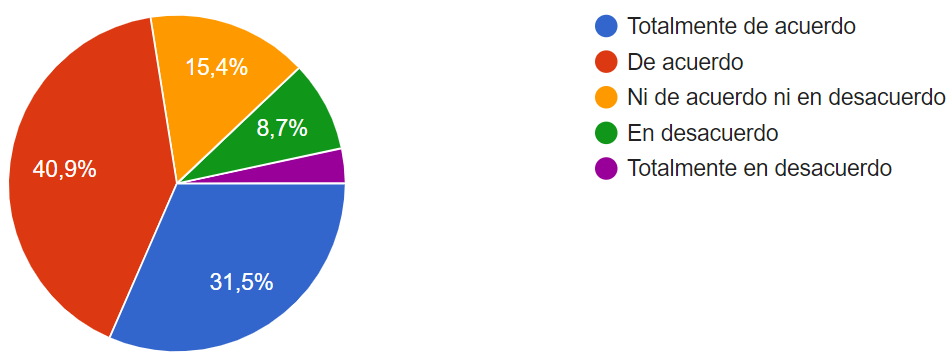
\includegraphics[width=0.8\textwidth]{resources/images/p1}
              \caption{Resultados de la encuesta en la pregunta uno}\label{fig:figure_p1}
    \end{figure}

\textbf{Análisis e interpretación:}\\
Los resultados de la pregunta uno muestran que el 31.5\% de los propietarios del conjunto habitacional {\textquotedblleft}El Portal de la Viña{\textquotedblright} están totalmente de acuerdo con el proceso actual para obtener la información de las obligaciones financieras de su domicilio, el 40.9\% de los propietarios están de acuerdo con el proceso actual, el 15.4\% de los propietarios ni están de acuerdo ni en desacuerdo con el proceso actual, el 8.7\% de los propietarios están en desacuerdo con el proceso actual y por último el 3.5\% de los propietarios están totalmente en desacuerdo con el proceso actual.
Tomando en cuenta los resultados obtenidos en la encuesta, se puede observar que el 72.4\% de los propietarios del conjunto habitacional consideran que el proceso actual para obtener la información de las obligaciones financieras de su domicilio es eficiente, mientras que, el 27.6\% de los propietarios consideran que el proceso actual no es eficiente y tomando en consideración las entrevistas realizadas a tesorería se concluye que se puede agilizar el proceso de consulta de información mediante el uso de una aplicación móvil.
\bigbreak

\textbf{Pregunta 2:} ¿Con que frecuencia solicita la información de las obligaciones financieras (pagos, multas, etc.) de su domicilio a tesorería?
    \begin{table}[H]
              \centering
              \caption{Resultados de la pregunta dos}
              \begin{tabular}{|c|c|c|}
                  \hline
                  \textbf{Indicador} & \textbf{Frecuencia} &  \textbf{Porcentaje} \\
                  \hline
                  Por lo menos una vez al mes & 135 & 90.6\% \\
                  \hline
                  Dos veces al mes & 5 & 3.4\% \\
                  \hline
                  Tres veces al mes
                  & 5 & 3.4\% \\
                  \hline
                  Cuatro veces al mes & 0 & 0\% \\
                  \hline
                  Más de cuatro veces al mes & 4 & 2.7\% \\
                  \hline
                  \textbf{Suma total} & 149 & 100\% \\
                  \hline
              \end{tabular}\label{tab:table_preg_2}
    \end{table}
    \begin{figure}[H]
              \centering
              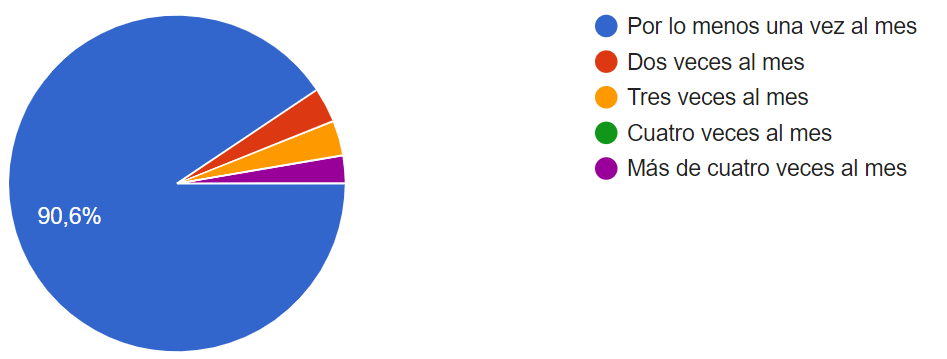
\includegraphics[width=0.8\textwidth]{resources/images/p2}
              \caption{Resultados de la encuesta en la pregunta dos}\label{fig:figure_p2}
    \end{figure}

\textbf{Análisis e interpretación:}\\
Los resultados de la pregunta dos evidencian que el 90.6\% de los propietarios del conjunto habitacional {\textquotedblleft}El Portal de la Viña{\textquotedblright} solicitan por lo menos una vez al mes la información de las obligaciones financieras de su domicilio a tesorería, el 3.4\% de los propietarios solicitan dos veces al mes, el 3.4\% de los propietarios solicitan tres veces al mes, el 0\% de los propietarios solicitan cuatro veces al mes y por último el 2.7\% de los propietarios solicitan más de cuatro veces al mes.
Por tanto, se puede observar que existe una demanda considerable de solicitudes a tesorería de manera mensual, lo cual junto con la entrevista realizada a tesorería se concluye que se puede facilitar el proceso de consulta de información mediante el uso de una aplicación móvil.

\bigbreak
\textbf{Pregunta 3:} ¿Cree usted que el proceso actual para el registro de asistencias durante la asamblea es eficiente en términos de tiempo?
    \begin{table}[H]
        \centering
        \caption{Resultados de la pregunta tres}
        \begin{tabular}{|c|c|c|}
            \hline
            \textbf{Indicador} & \textbf{Frecuencia} &  \textbf{Porcentaje} \\
            \hline
            Totalmente de acuerdo & 29 & 19.5\% \\
            \hline
            De acuerdo & 55 & 36.9\% \\
            \hline
            Ni de acuerdo ni en desacuerdo & 34 & 22.8\% \\
            \hline
            En desacuerdo & 17 & 11.4\% \\
            \hline
            Totalmente en desacuerdo & 14 & 9.4\% \\
            \hline
            \textbf{Suma total} & 149 & 100\% \\
            \hline
        \end{tabular}\label{tab:table_preg_3}
    \end{table}
    \begin{figure}[H]
        \centering
        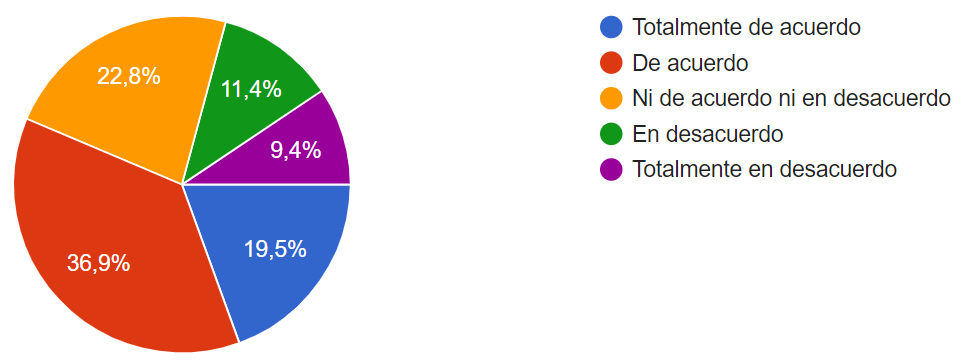
\includegraphics[width=0.8\textwidth]{resources/images/p3}
        \caption{Resultados de la encuesta en la pregunta tres}\label{fig:figure_p3}
    \end{figure}

\textbf{Análisis e interpretación:}\\
Los resultados de la pregunta tres muestran que el 19.5\% de los propietarios del conjunto habitacional {\textquotedblleft}El Portal de la Viña{\textquotedblright} están totalmente de acuerdo con el proceso actual para el registro de asistencias durante la asamblea, el 36.9\% de los propietarios están de acuerdo con el proceso actual, el 22.8\% de los propietarios ni están de acuerdo ni en desacuerdo con el proceso actual, el 11.4\% de los propietarios están en desacuerdo con el proceso actual y por último el 9.4\% de los propietarios están totalmente en desacuerdo con el proceso actual.
Por lo tanto, se observa que el 56.4\% de los propietarios del conjunto habitacional consideran que el proceso actual para el registro de asistencias durante la asamblea es eficiente en términos de tiempo, mientras que el 43.6\% de los propietarios consideran que el proceso actual no es eficiente y tomando en consideración las entrevistas realizadas a presidencia se concluye que se puede optimizar el proceso de registro de asistencias mediante el uso de sistemas informáticos.
\bigbreak
\textbf{Pregunta 4:} ¿Considera usted que el conteo actual de las votaciones durante las asambleas es transparente y eficiente?
    \begin{table}[H]
        \centering
        \caption{Resultados de la pregunta cuatro}
        \begin{tabular}{|c|c|c|}
            \hline
            \textbf{Indicador} & \textbf{Frecuencia} &  \textbf{Porcentaje} \\
            \hline
            Totalmente de acuerdo & 50 & 33.6\% \\
            \hline
            De acuerdo & 57 & 38.3\% \\
            \hline
            Ni de acuerdo ni en desacuerdo & 31 & 20.8\% \\
            \hline
            En desacuerdo & 5 & 3.4\% \\
            \hline
            Totalmente en desacuerdo & 6 & 4\% \\
            \hline
            \textbf{Suma total} & 149 & 100\% \\
            \hline
        \end{tabular}\label{tab:table_preg_4}
    \end{table}
    \begin{figure}[H]
        \centering
        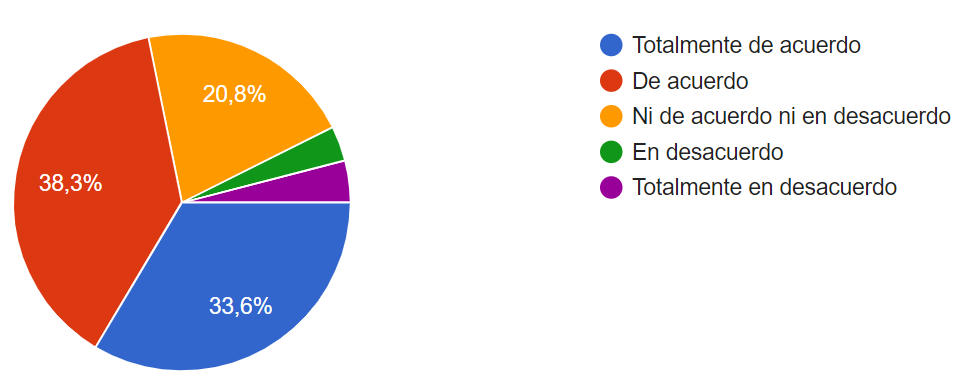
\includegraphics[width=0.8\textwidth]{resources/images/p4}
        \caption{Resultados de la encuesta en la pregunta cuatro}\label{fig:figure_p4}
    \end{figure}

\textbf{Análisis e interpretación:}\\
Los resultados de la pregunta cuatro muestran que el 33.6\% de los propietarios del conjunto habitacional {\textquotedblleft}El Portal de la Viña{\textquotedblright} están totalmente de acuerdo con el conteo actual de las votaciones durante las asambleas, el 38.3\% de los propietarios están de acuerdo con el conteo actual, el 20.8\% de los propietarios ni están de acuerdo ni en desacuerdo con el conteo actual, el 3.4\% de los propietarios están en desacuerdo con el conteo actual y por último el 4\% de los propietarios están totalmente en desacuerdo con el conteo actual.
Por lo cual, se puede observar que el 71.9\% de los propietarios del conjunto habitacional consideran que el conteo actual de las votaciones durante las asambleas es transparente y eficiente, mientras que el 28.1\% de los propietarios consideran que el conteo actual no es transparente y eficiente y tomando en consideración las entrevistas realizadas a presidencia en donde se expuso que la duración de las mismas suelen ser de entre veinte a treinta minutos, se concluye que se puede sistematizar el proceso de conteo de votaciones mediante el uso de sistemas informáticos para reducir y cumplir así con los tiempos establecidos de duración de las asambleas.
\bigbreak
\textbf{Pregunta 5:} ¿Ha experimentado retrasos en la entrega de los comprobantes de pagos?
    \begin{table}[H]
        \centering
        \caption{Resultados de la pregunta cinco}
        \begin{tabular}{|c|c|c|}
            \hline
            \textbf{Indicador} & \textbf{Frecuencia} &  \textbf{Porcentaje} \\
            \hline
            Si & 62 & 41.6\% \\
            \hline
            No & 87 & 58.4\% \\
            \hline
            \textbf{Suma total} & 149 & 100\% \\
            \hline
        \end{tabular}\label{tab:table_preg_5}
    \end{table}
    \begin{figure}[H]
        \centering
        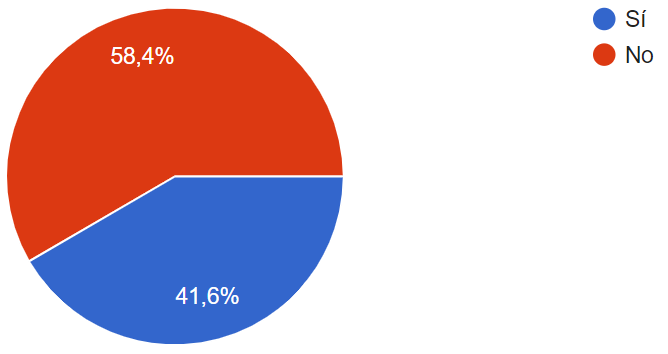
\includegraphics[width=0.8\textwidth]{resources/images/p5}
        \caption{Resultados de la encuesta en la pregunta cinco}\label{fig:figure_p5}
    \end{figure}

\textbf{Análisis e interpretación:}\\
Los resultados de la pregunta cinco muestran que el 41.6\% de los propietarios del conjunto habitacional {\textquotedblleft}El Portal de la Viña{\textquotedblright} han experimentado retrasos en la entrega de los comprobantes de pagos, mientras que el 58.4\% de los propietarios no han experimentado retrasos en la entrega de los comprobantes de pagos.
Por tanto, se evidencia que un sistema informático administrativo puede ser de gran ayuda para la directiva del conjunto habitacional, ya que se puede sistematizar el proceso de entrega de comprobantes de pagos y evitar retrasos en la entrega de los mismos.
\bigbreak
\textbf{Pregunta 6:} ¿Con qué frecuencia olvida que el pago de alícuotas de su domicilio esta por vencer?
    \begin{table}[H]
        \centering
        \caption{Resultados de la pregunta seis}
        \begin{tabular}{|c|c|c|}
            \hline
            \textbf{Indicador} & \textbf{Frecuencia} &  \textbf{Porcentaje} \\
            \hline
            Muy frecuentemente & 21 & 14.1\% \\
            \hline
            Frecuentemente & 20 & 13.4\% \\
            \hline
            Ocasionalmente & 31 & 20.8\% \\
            \hline
            Raramente & 36 & 24.2\% \\
            \hline
            Nunca & 41 & 27.5\% \\
            \hline
            \textbf{Suma total} & 149 & 100\% \\
            \hline
        \end{tabular}\label{tab:table_preg_6}
    \end{table}
    \begin{figure}[H]
        \centering
        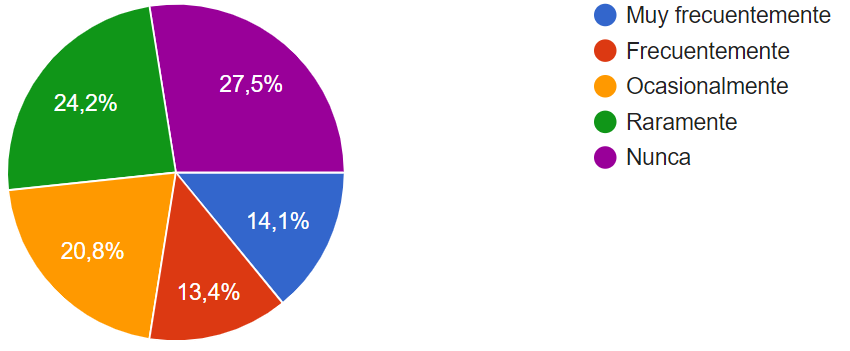
\includegraphics[width=0.8\textwidth]{resources/images/p6}
        \caption{Resultados de la encuesta en la pregunta seis}\label{fig:figure_p6}
    \end{figure}

\textbf{Análisis e interpretación:}\\
Los resultados de la pregunta seis muestran que el 14.1\% de los propietarios del conjunto habitacional {\textquotedblleft}El Portal de la Viña{\textquotedblright} olvidan muy frecuentemente que el pago de alícuotas de su domicilio están por vencer, el 13.4\% de los propietarios olvidan frecuentemente, el 20.8\% de los propietarios olvidan ocasionalmente, el 24.2\% de los propietarios olvidan raramente y por último el 27.5\% de los propietarios nunca olvidan que el pago de alícuotas.
Para mejorar estos resultados se puede implementar recordatorios de pagos por vencer mediante una aplicación móvil, ya que se evidencia que el 48.3\% de los propietarios lo olvidan muy frecuentemente, frecuentemente u ocasionalmente.
\bigbreak
\textbf{Pregunta 7:} ¿Con qué frecuencia ha utilizado el buzón de quejas/sugerencias?
    \begin{table}[H]
        \centering
        \caption{Resultados de la pregunta siete}
        \begin{tabular}{|c|c|c|}
            \hline
            \textbf{Indicador} & \textbf{Frecuencia} &  \textbf{Porcentaje} \\
            \hline
            Nunca lo he usado & 142 & 95.3\% \\
            \hline
            Al menos una vez al mes & 6 & 4\% \\
            \hline
            Dos veces al mes & 0 & 0\% \\
            \hline
            Tres veces al mes & 0 & 0\% \\
            \hline
            Más de tres veces al mes & 1 & 0.7\% \\
            \hline
            \textbf{Suma total} & 149 & 100\% \\
            \hline
        \end{tabular}\label{tab:table_preg_7}
    \end{table}
    \begin{figure}[H]
        \centering
        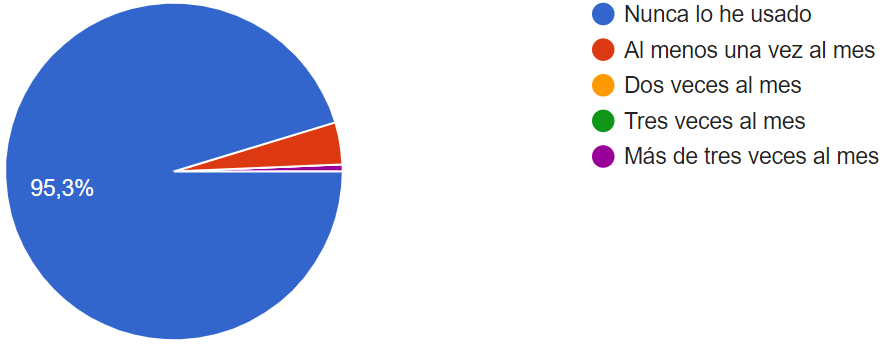
\includegraphics[width=0.8\textwidth]{resources/images/p7}
        \caption{Resultados de la encuesta en la pregunta siete}\label{fig:figure_p7}
    \end{figure}

\textbf{Análisis e interpretación:}\\
Los resultados de la pregunta siete muestran que el 95.3\% de los propietarios del conjunto habitacional {\textquotedblleft}El Portal de la Viña{\textquotedblright} nunca han utilizado el buzón de quejas/sugerencias, el 4\% de los propietarios lo han utilizado al menos una vez al mes, el 0\% de los propietarios lo han utilizado dos veces al mes, el 0\% de los propietarios lo han utilizado tres veces al mes y por último el 0.7\% de los propietarios lo han utilizado más de tres veces al mes.
Por tanto, se evidencia que el buzón de quejas/sugerencias no es utilizado por los propietarios del conjunto habitacional, lo cual se puede mejorar mediante una aplicación móvil que permita a los propietarios enviar sus quejas y sugerencias de una manera más sencilla y eficiente.
\bigbreak
\textbf{Pregunta 8:} ¿Considera usted que los medios actuales (WhatsApp/pizarrón en la garita) que utiliza la directiva para publicar comunicados son eficientes?

    \begin{table}[H]
        \centering
        \caption{Resultados de la pregunta ocho}
        \begin{tabular}{|c|c|c|}
            \hline
            \textbf{Indicador} & \textbf{Frecuencia} &  \textbf{Porcentaje} \\
            \hline
            Totalmente de acuerdo & 58 & 38.9\% \\
            \hline
            De acuerdo & 68 & 45.6\% \\
            \hline
            Ni de acuerdo ni en desacuerdo & 12 & 8.1\% \\
            \hline
            En desacuerdo & 4 & 2.7\% \\
            \hline
            Totalmente en desacuerdo & 7 & 4.7\% \\
            \hline
            \textbf{Suma total} & 149 & 100\% \\
            \hline
        \end{tabular}\label{tab:table_preg_8}
    \end{table}
    \begin{figure}[H]
        \centering
        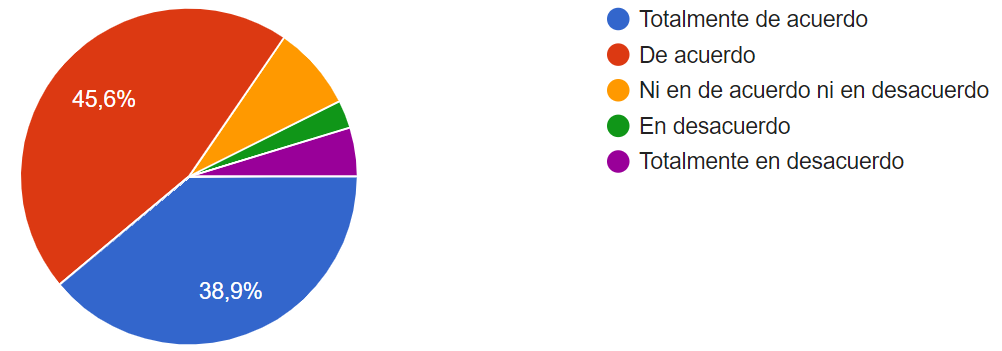
\includegraphics[width=0.8\textwidth]{resources/images/p8}
        \caption{Resultados de la encuesta en la pregunta ocho}\label{fig:figure_p8}
    \end{figure}

\textbf{Análisis e interpretación:}\\
Los resultados de la pregunta ocho muestran que el 38.9\% de los propietarios del conjunto habitacional {\textquotedblleft}El Portal de la Viña{\textquotedblright} están totalmente de acuerdo con los medios actuales que utiliza la directiva para publicar comunicados, el 45.6\% de los propietarios están de acuerdo con los medios actuales, el 8.1\% de los propietarios ni están de acuerdo ni en desacuerdo con los medios actuales, el 2.7\% de los propietarios están en desacuerdo con los medios actuales y por último el 4.7\% de los propietarios están totalmente en desacuerdo con los medios actuales.
Para mejorar estos resultados se puede implementar un sistema informático que permita a la directiva publicar comunicados de una manera más centralizada, ya que tomando en consideración las entrevistas realizadas a la directiva el uso de WhatsApp no es apto para la publicación de comunicados por el mal uso que le dan los demás residentes y el pizarrón en la garita no es visible para todos los propietarios.
\bigbreak
\textbf{Pregunta 9:} ¿Preferiría utilizar una aplicación móvil que le permita revisar la información de las obligaciones financieras de su domicilio, el registro de su asistencia y voto durante las asambleas, se le envíen notificaciones recordándole los pagos por vencer o que ha sido multado por alguna infracción?
    \begin{table}[H]
        \centering
        \caption{Resultados de la pregunta nueve}
        \begin{tabular}{|c|c|c|}
            \hline
            \textbf{Indicador} & \textbf{Frecuencia} &  \textbf{Porcentaje} \\
            \hline
            Si & 127 & 85.2\% \\
            \hline
            No & 22 & 14.8\% \\
            \hline
            \textbf{Suma total} & 149 & 100\% \\
            \hline
        \end{tabular}\label{tab:table_preg_9}
    \end{table}
    \begin{figure}[H]
        \centering
        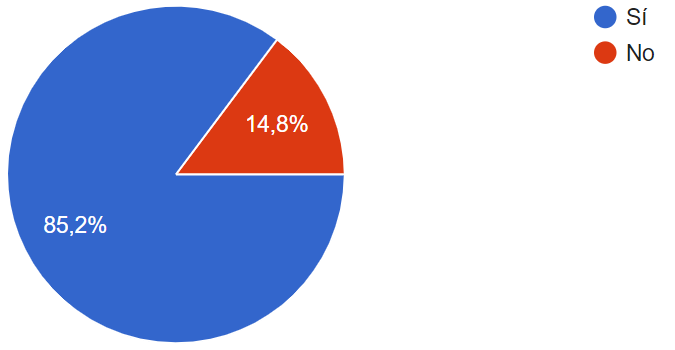
\includegraphics[width=0.8\textwidth]{resources/images/p9}
        \caption{Resultados de la encuesta en la pregunta nueve}\label{fig:figure_p9}
    \end{figure}

\textbf{Análisis e interpretación:}\\
Los resultados de la pregunta nueve muestran que el 85.2\% de los propietarios del conjunto habitacional {\textquotedblleft}El Portal de la Viña{\textquotedblright} preferirían utilizar una aplicación móvil que les permita revisar la información de las obligaciones financieras de su domicilio, el registro de su asistencia y voto durante las asambleas, se les envíen notificaciones recordándoles los pagos por vencer o que han sido multados por alguna infracción, mientras que el 14.8\% de los propietarios no preferirían utilizar una aplicación móvil.


\subsection{Procesamiento y análisis de datos}\label{subsec:procesamiento-y-analisis-de-datos}

Con la información recolectada a través de las entrevistas y las encuestas se concluyó que:
\begin{itemize}
    \item Actualmente la directiva lleva mucho de sus procesos de forma manual o en hojas de cálculo que han ocasionado atrasos y una alta carga de trabajo para todos los miembros de la misma.
    Los procesos administrativos actualmente funcionan, pero no son eficientes.
    Cada uno de los miembros de la directiva tienen sus funciones específicas, pero no cuentan con un sistema que les permita realizarlos de una manera más sencilla, puesto que todos ellos tienen empleos y no pueden dedicarle todo el tiempo que quisieran al conjunto habitacional.
    \item En presidencia se lleva a cabo el control y manejo de los parqueaderos de una manera manual y muy tediosa, debido a que deben de dibujar un croquis manual de los parqueaderos y actualizar las hojas de excel con los datos de los propietarios. El tiempo empleado en las asambleas es demasiado extenso, por el motivo de que se debe hacer el registro de asistencia por cada residente de manera manual en una hoja impresa.
    \item En tesorería se maneja la información económica del conjunto en hojas de cálculo, teniendo en cuenta que son 303 casas y 275 parqueaderos en total, se convierte en un problema muy alto en cuanto a la cantidad de información que se debe manejar y el tiempo que se debe emplear en la generación de reportes. Además lo anteriormente mencionado provoca atrasos en la entrega de recibos de pagos.
    \item En secretaría se lleva la generación de gran parte de actas y convocatorías mediante el uso de Word o Canva, en donde se identificó que estos documentos son generados de forma manual y para emitirlos se utiliza WhatsApp. Como consecuencía de esto los propietarios no suelen enterarse de las convocatorías ya que el grupo de  WhatsApp esta en gran parte del tiempo con mensajes irrelevantes y discusiones entre vecinos.
    \item De las encuestas realizadas a los propietarios se pudo identificar que la mayoría están conformes con la gestión de la directiva, sin embargo, se
     evidenció que los atrasos en las entregas de recibos de pagos es un problema bastante común. También existe un poco uso del buzón de sugerencias, ya que los propietarios prefieren comunicarse directamente con los miembros de la directiva. Y por último existe una necesidad alta de poder tener una aplicación móvil que les permite consultar información de su domicilio y notificar de eventos importantes.
\end{itemize}

\chapter{RESULTADOS Y DISCUSIÓN}\label{ch:resultados-y-discusion}
\section{Análisis de herramientas de desarrollo}\label{sec:analisis-frameworks-desarrollo}

En la siguiente sección se detalla el análisis de las herramientas de desarrollo que se utilizarán para la implementación del sistema de gestión de conjunto habitacional tanto frameworks como herramientas y metodologías de desarrollo que mejor se adapten a las necesidades del proyecto.

\subsection{Análisis y selección de frameworks}\label{subsec:analisis-seleccion-frameworks-desarrollo}

Dado que el sistema administrativo para la directiva será un sistema web y el sistema para los propietarios e inquilinos será un sistema móvil, se debe seleccionar un framework de desarrollo web, un framework de desarrollo móvil, un framework de desarrollo de APIs, un gestor de bases de datos y herramientas para la geolocalización.

\subsubsection{Framework de desarrollo web}\label{subsubsec:framework-desarrollo-web}

En primera instancia se debe evaluar las características de los frameworks de desarrollo web más utilizados en la actualidad, como Angular, React y Vue, para seleccionar el que mejor se adapte a las necesidades del proyecto.
Para lo cual en \cite{wu_desarrollo_2014}  el autor muestra una tabla de comparación entre las características de los frameworks de desarrollo web Angular, React y Vue que se detallan a continuación.

\begin{footnotesize}
\begin{spacing}{1}
    \begin{center}

        \renewcommand*{\arraystretch}{1.4}
        \begin{longtable}[c]{ |>{\bfseries}p{0.2\textwidth} |p{0.2\textwidth} |p{0.2\textwidth}  |p{0.2\textwidth}|  }
            \caption[Características de los framework front-end Angular, React y Vue]{ Características de los framework front-end Angular, React y Vue\cite{wu_desarrollo_2014} } \\
            \hline
            \multicolumn{1}{|c|}{ \textbf{Característica}} & \multicolumn{1}{c|}{\textbf{Angular}} & \multicolumn{1}{c|}{ \textbf{React}} & \multicolumn{1}{c|}{ \textbf{Vue}} \\
            \hline
            Tipo                                         & Framework                        & Biblioteca                  & Framework                     \\
            \hline
            Año de lanzamiento                           & 2016                                 & 2013                                & 2014                              \\
            \hline
            Lenguaje de programación                     & TypeScript                           & JavaScript                          & JavaScript                        \\
            \hline
            Tamaño del ecosistema                        & Grande                               & Grande                              & Mediano                           \\
            \hline
            Enlace de datos bidireccional                & Sí                                   & Sí                                  & Sí                                \\
            \hline
            Arquitectura de componentes                  & Sí                                   & Sí                                  & Sí                                \\
            \hline
            DOM Virtual                                  & No                                   & Sí                                  & Sí                                \\
            \hline
            Curva de aprendizaje                         & Relativamente pronunciada            & Moderada                            & Moderada                          \\
            \hline
            Rendimiento                                  & Bueno                                & Muy Bueno                           & Bueno                             \\
            \hline
            Soporte comunitario                          & Fuerte                               & Fuerte                              & Fuerte                            \\
            \hline
            Casos de uso                                 & Aplicaciones grandes y complejas     & Varias escalas                      & Varias escalas                    \\
            \hline
        \end{longtable}\label{tab:table_angular_react_vue_caracteristicas}

    \end{center}
\end{spacing}
\end{footnotesize}

En la Tabla \ref{tab:table_angular_react_vue_ventajas_desventajas} analizan también las ventajas y desventajas de los frameworks de desarrollo web Angular, React y Vue.
En donde el autor \cite{wu_desarrollo_2014}  realiza una extracción de las ventajas y desventajas de los frameworks los cuales serán detallados a continuación.

\begin{footnotesize}
\begin{spacing}{1}
    \begin{center}
        \renewcommand*{\arraystretch}{1.4}
        \begin{longtable}[c]{ |>{\bfseries}p{0.05\textwidth} |p{0.38\textwidth} |p{0.38\textwidth}|    }
            \caption[Ventajas y desventajas de los framework front-end Angular, React y Vue]{ Ventajas y desventajas de los framework front-end Angular, React y Vue\cite{wu_desarrollo_2014} }\label{tab:table_angular_react_vue_ventajas_desventajas} \\
            \hline
            \multicolumn{1}{|c|}{ \textbf{Framework}} & \multicolumn{1}{c|}{\textbf{Ventajas}} & \multicolumn{1}{c|}{ \textbf{Desventajas}} \\
            \hline
            Angular & \begin{itemize}
                          \item Potente
                          \item Vinculación de datos bidireccional
                          \item Arquitectura de componentes
                          \item Enrutamiento y navegación
                          \item Desarrollo multiplataforma
            \end{itemize}
            & \begin{itemize}
                  \item Curva de aprendizaje pronunciada
                  \item Grande y complejo
                  \item Problemas de rendimiento
                  \item No es optimo para proyectos pequeños
                  \item Escalabilidad adecuada para proyectos grandes
            \end{itemize} \\
            \hline
            React & \begin{itemize}
                        \item Alto rendimiento
                        \item Desarrollo por componentes
                        \item Comunidad activa
                        \item Ecosistema rico
            \end{itemize}
            & \begin{itemize}
                  \item Curva de aprendizaje alta para principiantes
                  \item Sintaxis JSX
                  \item Enfoque solo en la capa visible
            \end{itemize} \\
            \hline
            Vue & \begin{itemize}
                      \item Fácil de aprender
                      \item Marco incremental
                      \item Responsive data binding
                      \item Desarrollo por componentes
                      \item Ecosistema rico
            \end{itemize}
            & \begin{itemize}
                  \item Ecosistema pequeño comparado con Angular y React
                  \item Menos soporte comunitario en comparación con Angular y React
                  \item Menos consistente que Angular
            \end{itemize} \\
            \hline
        \end{longtable}
    \end{center}
\end{spacing}
\end{footnotesize}
Después de analizar las características, ventajas y desventajas de los frameworks de desarrollo web Angular, React y Vue, se selecciona el framework de desarrollo web Angular, ya que es el que mejor se adapta a las necesidades del proyecto debido a que proporciona un framework muy completo con una arquitectura ya predefinida además de tener una variedad de herramientas y librerías que facilitan el desarrollo de aplicaciones web y teniendo en cuenta que posee un framework de desarrollo móvil llamado Ionic que facilita la creación de aplicaciones móviles multiplataforma.

\subsubsection{Framework de desarrollo móvil}\label{subsubsec:framework-desarrollo-movil}

Como framework de desarrollo móvil se selecciona el framework de desarrollo móvil Ionic, ya que en el estudio comparativo en \cite{ahmad_analysis_2023}, el autor muestra una Tabla \ref{tab:table_movil_frameworks_comparacion} de resultados en donde se tiene en cuenta diversos factores de rendimiento, seguridad, facilidad de acceso al hardware, uso de CPU, uso de memoria, entre otros factores, en donde se evidencia que el framework de desarrollo móvil Ionic obtiene un puntaje de 81 puntos, React Native 85 puntos y Flutter 79 puntos.

\begin{footnotesize}
\begin{spacing}{1}

        \begin{center}
            \renewcommand*{\arraystretch}{1.4}
            \begin{longtable}[c]{ |>{\bfseries}p{0.15\textwidth}  |p{0.05\textwidth} |p{0.05\textwidth}  |p{0.05\textwidth}  |p{0.05\textwidth}  |p{0.05\textwidth}  |p{0.05\textwidth}|   }
                \caption[Comparación de los frameworks: Métricas y puntuajes]{ Comparación de los frameworks: Métricas y puntuajes \cite{ahmad_analysis_2023}}\label{tab:table_movil_frameworks_comparacion} \\
                \hline
                \multicolumn{1}{|c|}{ \textbf{Métrica}}  & \multicolumn{1}{c|}{\textbf{Ionic}} & \multicolumn{1}{c|}{ \textbf{React Native}} & \multicolumn{1}{c|}{ \textbf{Flutter}} & \multicolumn{1}{c|}{ \textbf{NativeScript}} & \multicolumn{1}{c|}{ \textbf{MAUI}} & \multicolumn{1}{c|}{ \textbf{ReactJs}}\\
                \hline
                Plataformas objetivo                   & \multicolumn{1}{c|}{10}             & \multicolumn{1}{c|}{10}                     & \multicolumn{1}{c|}{10} & \multicolumn{1}{c|}{6}  & \multicolumn{1}{c|}{8} & \multicolumn{1}{c|}{10} \\
                \hline
                Acceso al hardware                     & \multicolumn{1}{c|}{13}             & \multicolumn{1}{c|}{16}                     & \multicolumn{1}{c|}{16} & \multicolumn{1}{c|}{14} & \multicolumn{1}{c|}{14} & \multicolumn{1}{c|}{16} \\
                \hline
                Funciones específicas de la plataforma & \multicolumn{1}{c|}{18}             & \multicolumn{1}{c|}{17} & \multicolumn{1}{c|}{18} & \multicolumn{1}{c|}{18} & \multicolumn{1}{c|}{16} & \multicolumn{1}{c|}{12} \\
                \hline
                Distribución de canales                & \multicolumn{1}{c|}{4}              & \multicolumn{1}{c|}{4}                      & \multicolumn{1}{c|}{4}  & \multicolumn{1}{c|}{4}  & \multicolumn{1}{c|}{4}  & \multicolumn{1}{c|}{1}  \\
                \hline
                Testeo                                 & \multicolumn{1}{c|}{8}              & \multicolumn{1}{c|}{8}                      & \multicolumn{1}{c|}{8}                 & \multicolumn{1}{c|}{4}  & \multicolumn{1}{c|}{8}  & \multicolumn{1}{c|}{8}  \\
                \hline
                Monetización                           & \multicolumn{1}{c|}{6}              & \multicolumn{1}{c|}{6}                      & \multicolumn{1}{c|}{6}                 & \multicolumn{1}{c|}{6}  & \multicolumn{1}{c|}{3}  & \multicolumn{1}{c|}{6}  \\
                \hline
                Integración personalizada de código    & \multicolumn{1}{c|}{2}              & \multicolumn{1}{c|}{2}                      & \multicolumn{1}{c|}{2}  & \multicolumn{1}{c|}{2}  & \multicolumn{1}{c|}{2}  & \multicolumn{1}{c|}{0}  \\
                \hline
                Seguridad                              & \multicolumn{1}{c|}{8}              & \multicolumn{1}{c|}{6}                      & \multicolumn{1}{c|}{6}                 & \multicolumn{1}{c|}{8}  & \multicolumn{1}{c|}{6}  & \multicolumn{1}{c|}{6}  \\
                \hline
                Uso del CPU                            & \multicolumn{1}{c|}{3}              & \multicolumn{1}{c|}{6}                      & \multicolumn{1}{c|}{2}                 & \multicolumn{1}{c|}{1}  & \multicolumn{1}{c|}{5}  & \multicolumn{1}{c|}{4}  \\
                \hline
                Uso de memoria                         & \multicolumn{1}{c|}{3}              & \multicolumn{1}{c|}{6}                      & \multicolumn{1}{c|}{2}  & \multicolumn{1}{c|}{1}  & \multicolumn{1}{c|}{5}  & \multicolumn{1}{c|}{4}  \\
                \hline
                Tamaño de la aplicación                & \multicolumn{1}{c|}{6}              & \multicolumn{1}{c|}{4}                      & \multicolumn{1}{c|}{5}  & \multicolumn{1}{c|}{2}  & \multicolumn{1}{c|}{1}  & \multicolumn{1}{c|}{3}  \\
                \hline
                \textbf{Total}                         & \multicolumn{1}{c|}{\textbf{81}}    & \multicolumn{1}{c|}{\textbf{85}}            & \multicolumn{1}{c|}{\textbf{79}}                           & \multicolumn{1}{c|}{\textbf{66}}                                & \multicolumn{1}{c|}{\textbf{72}}                        & \multicolumn{1}{c|}{\textbf{70}}                           \\
                \hline
            \end{longtable}
        \end{center}

\end{spacing}
\end{footnotesize}

Por lo cual teniendo en consideración de que Ionic es un framework que en puede trabajar con Angular el cual también se utilizará para el desarrollo web y los resultados obtenidos del estudio revisado en donde se evidencia que Ionic tiene un buen rendimiento en las métricas medidas siendo únicamente superada por React Native por 4 puntos se elige el framework de desarrollo móvil Ionic.

\subsubsection{Framework de desarrollo back-end}

Dado que el proyecto será tanto web como móvil se realizará un estudio comparativo de frameworks que faciliten la creación de una API para comunicar tanto interfaz de usuario web como la interfaz de usuario móvil con la base de datos.
\bigbreak

Como lenguaje de programación se selecciona Java, ya que en \cite{zhang_design_2021}, el autor menciona que java es un lenguaje muy robusto y seguro, orientado a objetos, con una amplia comunidad, además el autor menciona que es más eficiente que lenguajes de programación muy usados como .NET en términos de tiempo de respuesta y utilización de recursos.
\bigbreak
En \cite{choma_efficiency_2023}, el autor realizó un estudio comparativo entre los frameworks de desarrollo back-end Spring Boot, Django y Express, en dicho estudio se les realizaron pruebas de rendimiento enviando dieciséis mil peticiones HTTP simultáneas de tipo GET, POST, PUT y DELETE, en donde se evidenció la superioridad de Spring Boot ya que el autor menciona que éste framework supera al resto debido a que implementa mejores mecanismos de mejoras de rendimiento extraídos de Spring Framework, por lo cual se selecciona este framework para el desarrollo back-end.
\bigbreak

\subsubsection{Herramienta de geolocalización}

Para la obtención de las ubicaciones en tiempo real se usara el plugin de geolocalización que viene integrado en Ionic, el cual esta provisto de métodos simples para obtener la ubicación actual y poder hacerle un seguimiento en tiempo real usando el GPS del dispositivo móvil \cite{ionic_geolocation}.
\bigbreak
Por otro lado, se usara la API de Google Maps para la visualización de las ubicaciones en un mapa, ya que esta API proporciona una variedad de herramientas para la visualización de mapas y la obtención de ubicaciones, además de funciones en la cuales nos permite representar áreas mediante la configuración de polígonos y círculos \cite{poligons}.


\subsubsection{Gestor de bases de datos}

Las bases de datos son un componente fundamental en el desarrollo de aplicaciones, por lo cual se debe seleccionar un gestor de bases de datos que se adapte a las necesidades del proyecto, en donde se debe tener en cuenta la escalabilidad, la seguridad, la disponibilidad y la facilidad de uso.

\begin{footnotesize}
\begin{spacing}{1}
    \begin{center}

        \renewcommand*{\arraystretch}{1.4}
        \begin{longtable}[c]{ |>{\bfseries}p{0.2\textwidth}| p{0.2\textwidth}| p{0.2\textwidth}|  p{0.2\textwidth}|  }
            \caption[Comparación entre gestores SQL, NoSQL y NewSQL]{ Comparación entre gestores SQL, NoSQL y NewSQL\cite{lasluisa_evaluacion_2020} }\label{tab:table_sql_nosql_newsql} \\
            \hline
            \multicolumn{1}{|c|}{ \textbf{Descripción}} & \multicolumn{1}{c|}{\textbf{Relacional}} & \multicolumn{1}{c|}{ \textbf{No Relacional}} & \multicolumn{1}{c|}{ \textbf{NewSQL}} \\
            \hline
            Modelo de datos & Normaliza los datos en
            tablas conformadas por filas y columnas.
            Define estrictamente relación entre tablas
            & Proporciona una variedad
            de modelos de datos,
            como pares clave/valor,
            documentos y gráficos.
            & Estructura de datos
            flexible en donde es
            posible combinar la
            transaccionalidad y alta
            redundancia. \\
            \hline
            Cargas de trabajo óptima & Están diseñadas para
            aplicaciones de procesamiento
            de transacciones online (OLTP)
            y procesamiento analítico
            online (OLAP). & Las bases de datos de
            búsqueda NoSQL están
            diseñadas para hacer
            análisis sobre datos
            semiestructurados.
            & Alto rendimiento para
            cargas de trabajo OLTP/
            OLAP. \\
            \hline
            Escalabilidad & Escalabilidad vertical,
            crecimiento de la cantidad
            de nodos de almacenamiento
            depende de la estructura
            tecnológica física.
            & Escalabilidad horizontal y
            se distribuye la carga por
            todos los nodos.
            & Escalabilidad horizontal
            proporcionando un alta
            rendimiento en una amplia
            gama de plataformas. \\
            \hline
            Propiedades ACID & Las bases de datos relacional
            ofrecen propiedades de
            atomicidad, coherencia,
            aislamiento y durabilidad
            (ACID). & Las bases de datos
            NoSQL hacen
            concesiones al
            flexibilizar algunas de las
            propiedades ACID para
            un modelo de datos más
            flexible.
            & Mantiene las propiedades
            de ACID de un sistema de
            base de datos tradicional o
            relacional. \\
            \hline
            Tolerancia a fallos & Fallo en el nodo generalmente
            hará fallar la consulta.
            & Configurados para que
            la perdida de algunos
            nodos no interrumpa
            funcionamiento global.
            & Crash Recovery: Las
            bases de datos NewSQL
            tienen un mecanismo
            que les permite recuperar
            datos y pasar a un estado
            coherente.\\
            \hline
        \end{longtable}

    \end{center}
\end{spacing}
\end{footnotesize}
\newpage
Una vez analizadas las características de los gestores descritos en la Tabla \ref{tab:table_sql_nosql_newsql}, se selecciona el gestor de bases de datos relacional, ya que son gestores en los cuales los datos están normalizados en tablas y se define estrictamente la relación entre tablas, además de que es un gestor de bases de datos que se adapta a las necesidades del proyecto, ya que Spring Boot tiene soporte para el ORM Hibernate que facilita la conexión y el manejo de la los datos.

\bigbreak

Como sistema de gestor de bases de datos relacional se elige PostgreSQL, ya que en \cite{leon_soberon_alisis_2020}, el autor realiza un análisis de los gestores de bases de datos PostgreSQL y MySQL obteniendo como resultado que PostgeSQL tiene un mejor resultado en términos de consumo de CPU y memoria sobre MySQL, sin embargo en los procesos CRUD(Create, Read, Update, Delete) de eliminar y consultar imágenes MySQL tiene un mejor rendimiento, por lo cual teniendo en cuenta que no se realizarán almacenamiento de imágenes en la base de datos se selecciona PostgreSQL.
\section{Definición de la metodología de desarrollo de software}\label{sec:definicion-metodologia}

En la siguiente sección se detalla la metodología de desarrollo de software que se utilizará para la implementación del sistema de gestión de conjunto habitacional.
La metodología de desarrollo de software es un enfoque estructurado para la creación de sistemas de software.
Existen dos tipos de metodologías de desarrollo de software: metodologías tradicionales y metodologías ágiles.
A continuación, se mostrará una comparación entre ambas metodologías y se justificará la elección de la metodología seleccionada para el desarrollo del sistema de gestión de conjunto habitacional.

\subsection{Comparación entre metodologías tradicionales y metodologías ágiles}\label{subsec:comparacion-entre-metodologias-tradicionales-y-metodologias-agiles}

En la tabla \ref{tab:table_agil_vs_tradicional} se muestra una comparación entre las metodologías ágiles y las metodologías tradicionales.
En donde se puede evidenciar que las metodologías ágiles se enfocan más en la adaptación de posibles cambios, en proyectos pequeños y con un equipo de trabajo pequeño junto con una buena colaboración entre el equipo de desarrollo y el cliente.
Por otro lado las metodologías tradicionales se evidencia su utilidad de aplicación en proyectos grandes, con un equipo de trabajo grande y con una planificación previa amplia.
Por el análisis previo se llegó a la conclusión que para llevar este proyecto a cabo se utilizará una metodología ágil, ya que se cuenta con un equipo de trabajo pequeño, con entregas continuas al cliente y con la posibilidad de adaptarse a los cambios que se presenten durante el desarrollo del sistema.
En \cite{islam_comparison_2020} se extrajo la siguiente tabla que compara las metodologías ágiles con las metodologías tradicionales.

\begin{table}[H]
    \centering
    \caption[Comparación entre metodologías ágiles y metodologías tradicionales]{Comparación entre metodologías ágiles y metodologías tradicionales traducido de \cite{islam_comparison_2020} }\label{tab:table_agil_vs_tradicional}
    \renewcommand*{\arraystretch}{1.4}
    \begin{footnotesize}
    \begin{tabular}{ |>{\bfseries}l|l|l| }
        \hline
        \multicolumn{1}{|c|}{ \textbf{Característica}} & \multicolumn{1}{c|}{\textbf{Metodologías Ágiles}} & \multicolumn{1}{c|}{ \textbf{Metodologías Tradicionales}} \\
        \hline
        Enfoque                                      & Adaptativo                                       & Predictivo                                               \\
        \hline
        Medición de éxito                            & Valor de negocio                                 & Conforme al plan                                         \\
        \hline
        Tamaño
        del proyecto                                & Pequeño                                           & Grande                                                   \\
        \hline
        Estilo de gestión                            & Descentralizado                                  & Autocrático                                              \\
        \hline
        Perspectiva de cambio                        & Adaptable                                        & Sostenible                                 \\
        \hline
        Cultura                                      & Liderazgo - Colaboración                         & Ordenar - Controlar                                      \\
        \hline
        Documentación                                & Baja                                             & Alta                                                     \\
        \hline
        Énfasis                                      & Orientado al cliente                             & Orientado al proceso                                     \\
        \hline
        Ciclos                                       & Numerosos                                        & Limitados                                                \\
        \hline
        Domínio                                      & Impredecible/Exploratorio                        & Predecible                                               \\
        \hline
        Planificación previa                         & Mínima                                           & Amplia                                                   \\
        \hline
        Retorno de la inversión                      & Principio del proyecto                           & Fin del proyecto                                         \\
        \hline
        Tamaño del equipo                            & Pequeño                                          & Grande                                                   \\
        \hline
    \end{tabular}
    \end{footnotesize}
\end{table}

Por otro lado para escoger la metodología ágil que se utilizará en el desarrollo del sistema de gestión de conjunto habitacional se realizó un análisis de las metodologías ágiles más utilizadas en la actualidad detalladas a continuación en la siguiente tabla.
En \cite{barriga_sanchez_sistema_2023} se extrajo la siguiente tabla que compara algunas de las metodologías ágiles más utilizadas en la actualidad.

\newpage
\begin{footnotesize}
\begin{spacing}{1}
    \begin{center}
        \renewcommand*{\arraystretch}{1.4}
        \begin{longtable}[l]{ |>{\bfseries}p{0.15\textwidth}| p{0.17\textwidth} |p{0.17\textwidth}  |p{0.17\textwidth} | p{0.17\textwidth}|}
            \caption[Comparación de las metodologías de desarrollo ágiles]{ Comparación de las metodologías de desarrollo ágiles\cite{barriga_sanchez_sistema_2023} }\label{tab:table_metodologias_agiles} \\
            \hline
            \multicolumn{1}{|c|}{ \textbf{Criterio}} & \multicolumn{1}{c|}{\textbf{XP}}                                                                        & \multicolumn{1}{c|}{ \textbf{Lean}} & \multicolumn{1}{c|}{ \textbf{RAD}}  & \multicolumn{1}{c|}{ \textbf{Kanban}}\\
            \hline
            Enfoque                                & Iterativo e incremental                                                                                & Iterativo e incremental                                                                        & Prototipado                                                                                & Continuo                                                                                \\
            \hline
            Principios                             & Integración continua, programación en pares, desarrollo basado en pruebas, comentarios de los clientes & Centrarse en el valor, eliminar desperdicios, flujo, mejora continua, respeto por las personas & Desarrollo rápido, participación del usuario, desarrollo iterativo, creación de prototipos & Visualización del flujo de trabajo, limitación del trabajo en progreso, mejora continua \\
            \hline
            Tamaño del equipo                      & 3--5                                                                                                   & 2--3                                                                                           & 2--3                                                                                       & No definido                                                                             \\
            \hline
            Tamaño del proyecto                    & Pequeños y medianos con requisitos bien definidos                                                      & Efectivo para proyectos grandes con requisitos complejos & Pequeños y medianos con requisitos cambiantes & Pequeños, medianos y grandes \\
            \hline
            Ventajas & Calidad y comunicación & Velocidad y flexibilidad & Costo y tiempo & Mejor flujo de trabajo \\
            \hline
            Simplicidad                            & Se busca la simplicidad en el código, en el diseño y en la solución de problemas & Se busca eliminar desperdicio y complejidad innecesaria para mejorar la eficiencia & Se enfoca en desarrollar soluciones simples y rápidas, evitando excesos de diseño & Busca eliminar desperdicio, simplificar procesos y claridad de flujo de trabajo \\
            \hline
            Entrega de software                    & Frecuente y regular                                                                                    & Entrega incremental                                                                            & Entrega rápida                                                                             & Entrega continua                                                                        \\
            \hline
            Planificación                          & Planificación continua                                                                                 & Planificación y modelado                                                                       & Planificación rápida y flexible & Planificación continua y visual \\
            \hline
        \end{longtable}

    \end{center}
\end{spacing}
\end{footnotesize}

Del análisis de la Tabla \ref{tab:table_metodologias_agiles} se llegó a la conclusión de que la metodología ágil que se utilizará en el desarrollo del proyecto será RAD, ya que se ajusta a las necesidades del proyecto, debido a que el equipo de desarrollo es pequeño, el proyecto es de tamaño mediano y se cuenta con tiempo limitado para la entrega del sistema.
Además, sus características de desarrollo rápido junto con la entrega de prototipos funcionales y participación del usuario, permitirá una mayor adaptabilidad a los cambios que se presenten durante el desarrollo del sistema.

\section{Cálculo de la distancia Haversine}\label{sec:calculo-de-la-distancia-haversine}

El cálculo de la distancia entre dos puntos geográficos es una tarea común en la programación de aplicaciones que requieren la ubicación de un usuario o la ubicación de un lugar específico.
En el caso de la aplicación móvil, se requiere conocer si el usuario se encuentra dentro de un rango de distancia de el lugar de reuniones en las asambleas de conjunto residencial.
\bigbreak
En \cite{camino_costa_desarrollo_2012} el autor menciona que la fórmula de Haversine es una fórmula utilizada para calcular la distancia entre dos puntos en la superficie de una esfera, en este caso, la Tierra.
Además, menciona que esta fórmula es precisa en el cálculo numérico incluso a distancias pequeñas, lo cual es ideal debido a que la precisión es un factor importante en la aplicación móvil, ya que será determinante para la verificación de la ubicación de los residentes.
\bigbreak
La fórmula de Haversine se define como:


\begin{itemize}
  \item $R$: Radio de la Tierra (aproximadamente 6371 km o 6371e3 metros).
  \item $\text{lat1}$, $\text{lon1}$: Latitud y longitud del primer punto en grados.
  \item $\text{lat2}$, $\text{lon2}$: Latitud y longitud del segundo punto en grados.
  \item $dLat$: Diferencia de latitud en radianes.
  \item $dLon$: Diferencia de longitud en radianes.
  \item $a$: Fórmula de Haversine.
  \item $c$: Ángulo central en radianes.
  \item $d$: Distancia entre los dos puntos en metros.
\end{itemize}


\begin{equation}
    \begin{aligned}
        \text{R} &= 6371e3 \\
        \text{dLat} &= \text{lat2} - \text{lat1} \\
        \text{dLon} &= \text{lon2} - \text{lon1} \\
        a &= \sin^2\left(\frac{dLat}{2}\right) + \cos(\text{lat1}) \cdot \cos(\text{lat2}) \cdot \sin^2\left(\frac{dLon}{2}\right) \\
        c &= 2 \cdot \text{atan2}\left(\sqrt{a}, \sqrt{1-a}\right) \\
        d &= R \cdot c \\
    \end{aligned}\label{eq:equation3}
\end{equation}






\section{Análisis del proceso actual}\label{sec:analisis-proceso-actual}

Para poder determinar el flujo del sistema se deben analizar los procesos actuales del conjunto habitacional, para ello se debe identificar los actividades que se llevan a cabo en el conjunto habitacional, los actores que intervienen en las mismas y los resultados que se obtienen.
Estos procesos fueron identificados en base a los resultados de las entrevistas y encuestas realizadas en el capítulo anterior.
\bigbreak
A continuación se muestran los procesos identificados en el conjunto habitacional:
\begin{itemize}
    \item Proceso de administración de parqueaderos.
    Proceso en el cual previamente revisada la documentación entregada de manera física del propietario o inquilino se le proporcionará un parqueadero de zona azul o particular dependiendo del tipo de parqueadero solicitado y siempre y cuando se cumpla con los requisitos establecidos en el reglamento del conjunto habitacional.
    \item Proceso de administración de eventos sociales.
    Proceso en el cual se lleva a cabo la organización de eventos sociales en el conjunto habitacional.
    \item Proceso de administración de guardianía.
    Proceso en el cual se lleva a cabo la administración de la guardianía del conjunto habitacional junto con las actividades que se realizan en la misma y los incidentes que se presentan.
    \item Proceso de administración de convocatorias.
    Proceso en el cual se lleva a cabo la organización de convocatorias en el conjunto habitacional, en donde en el caso de ser asambleas se registra la asistencia de los propietarios o inquilinos y se lleva a cabo la votación de las propuestas.
    \item Proceso de administración financiera.
    Proceso en el cual se administran los recursos financieros del conjunto habitacional tanto los ingresos como los egresos, multas y los proveedores.
    \item Proceso de administración de áreas comunales.
    Proceso en el cual se lleva a cabo la gestión del mantenimiento de las áreas comunales del conjunto habitacional tales como la limpieza y cortes de césped.
    \item Proceso de administración de la bitácora de la directiva.
    Proceso en el cual se lleva a cabo el registro de las actividades realizadas por la directiva del conjunto habitacional.
    \item Proceso de generación de documentos.
    Proceso en el cual se lleva a cabo la generación de documentos para los propietarios o inquilinos del conjunto habitacional.
    \item Proceso de consulta obligaciones financieras.
    Proceso en el cual se lleva a cabo la consulta de información de las obligaciones financieras de los propietarios o inquilinos del conjunto habitacional.
    \item Proceso de registro de asistencias en asambleas.
    Proceso en el cual cada propietario o inquilino del conjunto habitacional registra su asistencia a las asambleas.
    \item Proceso de votación en asambleas.
    Proceso en el cual únicamente los propietarios del conjunto habitacional realizan la votación de los temas a tratar en las asambleas.
\end{itemize}

De los procesos mencionados anteriormente se establecieron cuatro procesos principales los cuales serán detallados a continuación:
\begin{itemize}
    \item Proceso de administración de parqueaderos (Zona azul).
    \begin{enumerate}
        \item El propietario o inquilino debe realizar una solicitud via telefónica o presencial al presidente de la directiva.
        \item Se verifica que el propietario o inquilino cumpla con los requisitos establecidos en el reglamento de parqueaderos.
        \begin{enumerate}
            \item Si cumple con los requisitos se procede al siguiente proceso.
            \item Si no cumple con los requisitos se finaliza el proceso.
        \end{enumerate}
        \item El presidente solicita enviar la documentación requerida para la asignación de un parqueadero.
        \begin{enumerate}
            \item Si entrega la documentación completa se procede al siguiente proceso.
            \item Si no entrega la documentación completa se finaliza el proceso.
        \end{enumerate}

        \item El inquilino debe realizar el pago por adelantado de 10\textdollar.
        \item Se verifica el pago realizado por el inquilino.
        \begin{enumerate}
            \item Si el pago es válido se procede al siguiente proceso.
            \item Si el pago no es válido se finaliza el proceso.
        \end{enumerate}
        \item Se registra el pago en el libro de ingresos.
        \item Se genera la orden de pago.
        \item Se registra al propietario o inquilino en el libro de parqueaderos.
        \item Se genera una carta de compromiso.
        \item Se entrega la orden de pago físicamente al inquilino y se le toma una foto como respaldo.
    \end{enumerate}
    \begin{figure}[H]
        \centering
        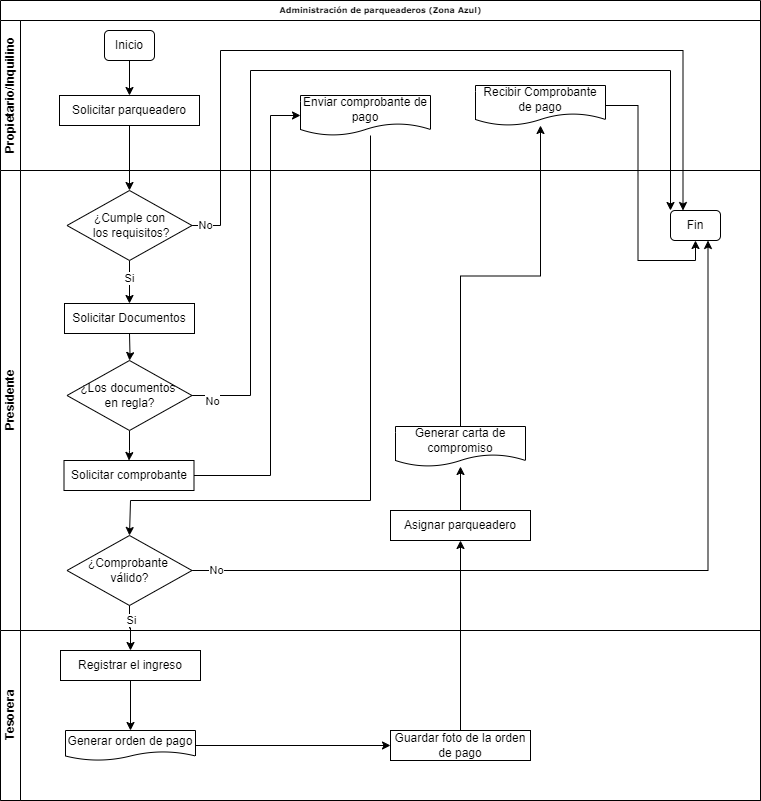
\includegraphics[width=1\textwidth]{resources/images/Diagramade flujo parqueadero-actual}
        \caption{Diagrama de flujo de procesos actual de administración de parqueaderos (Zona azul).}
        \label{fig:flujo-proceso-actual-parqueadero-azul}
    \end{figure}
    \item Proceso de administración de convocatorias.
    \begin{enumerate}
        \item La directiva del conjunto se reúne para definir la fecha de la convocatoria.
        \item Se crea la publicación de la convocatoria y se comparte en los medios de comunicación del conjunto habitacional.
        \item Se reenvía la publicación como recordatoria una semana antes de darse la convocatoria solo si es de asambleas.
        \item Se lleva a cabo la convocatoria.
        \begin{itemize}
            \item Si es una asamblea se procede al siguiente proceso.
            \item Si es una reunión o sesión de directiva se salta al proceso 6.
        \end{itemize}
        \item Se registra la asistencia de los propietarios o inquilinos.
        \item Se tratan los temas de la convocatoria.
        \item Se propone una votación de los temas a tratar.
        \begin{itemize}
            \item Si existe una votación se procede al siguiente proceso.
            \item Si no existe una votación se salta al proceso 9.
        \end{itemize}
        \item Se lleva a cabo el conteo de votos a mano alzada únicamente de propietarios.
        \item Se notifica a los propietarios el resultado de la votación.
        \item Se finaliza la convocatoria.
        \item Se genera el informe de asistencia.
        \item Se genera el acta de la convocatoria.
        \begin{itemize}
            \item Si es una asamblea se procede al siguiente proceso.
            \item Si es una reunión o sesión de directiva se finaliza el proceso.
        \end{itemize}
        \item Se envía el informe de asistencia a los residentes y se registra la respectiva multa.
        \item El propietario o inquilino puede presentar una justificación por la inasistencia en las siguientes 24 horas.
        \item Se verifica la justificación presentada.
        \begin{itemize}
            \item Si la justificación es válida se procede a eliminar la multa y termina el proceso.
            \item Si la justificación no es válida la multa se mantiene y termina el proceso.
        \end{itemize}
    \end{enumerate}

    \begin{figure}[H]
              \centering
              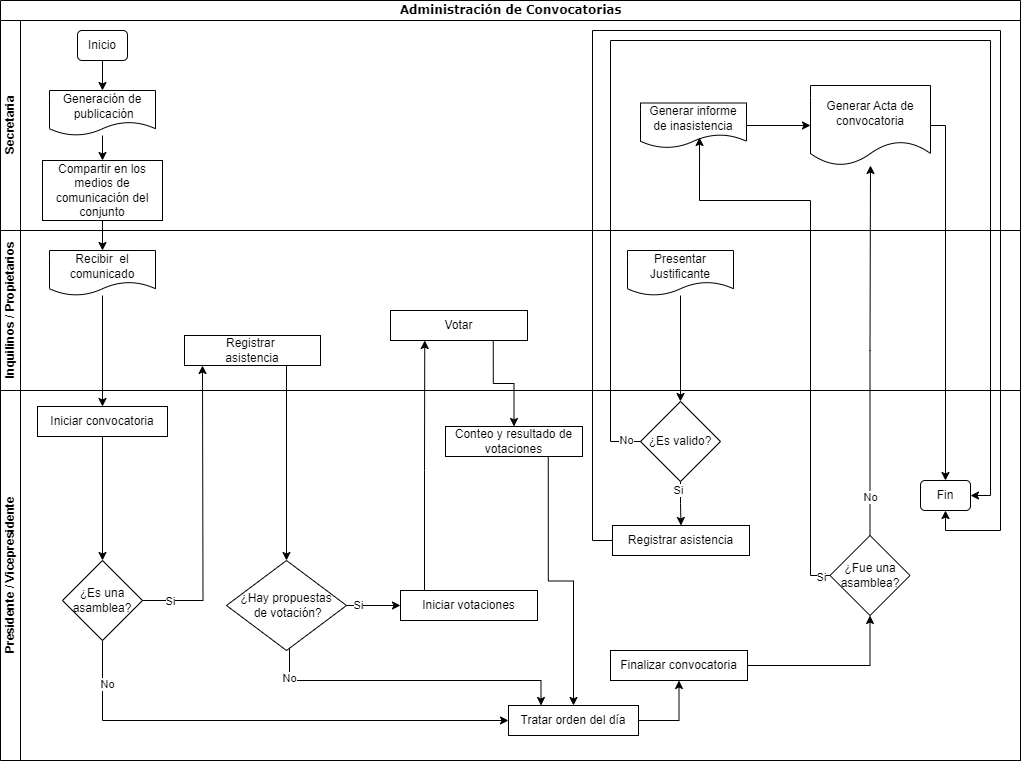
\includegraphics[width=1\textwidth]{resources/images/Copia de Diagrama de flujo convocatorias-actual}
              \caption{Diagrama de flujo de procesos actual de administración de convocatorias.}
              \label{fig:flujo-proceso-actual-convocatorias}
    \end{figure}
    \item Proceso de administración financiera.
    \begin{enumerate}
        \item Pagos de obligaciones financieras mensuales
        \begin{enumerate}
            \item El inquilino realiza el pago de la mensualidad de sus obligaciones financieras.
            \item El inquilino envía el comprobante de pago a la tesorera.
            \item La tesorera verifica el comprobante de pago.
            \begin{itemize}
                \item Si el comprobante es válido se procede al siguiente proceso.
                \item Si el comprobante no es válido se finaliza el proceso.
            \end{itemize}
            \item La tesorera revisa la última fecha de pago del inquilino.
            \item Se registra el pago en el libro de ingresos.
            \item Se genera una orden de pago.
            \item La tesorera entrega la orden de pago a guardianía pára que se le entregue al inquilino.
        \end{enumerate}
        \begin{figure}[H]
            \centering
            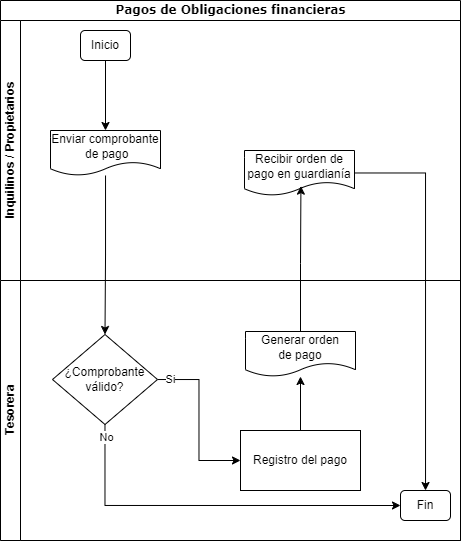
\includegraphics[width=1\textwidth]{resources/images/Diagrama de flujo de proceso pagos obligaciones actual}
            \caption{Diagrama de flujo de procesos actual del pago de obligaciones financieras.}
            \label{fig:flujo-proceso-actual-pagos-obligaciones-financieras}
        \end{figure}
        \item Pagos a proveedores
        \begin{enumerate}
            \item El proveedor envía la factura a la tesorera.
            \item La tesorera verifica la factura.
            \begin{itemize}
                \item Si la factura es válida se procede al siguiente proceso.
                \item Si la factura no es válida se finaliza el proceso.
            \end{itemize}
            \item La tesorera registra la factura en el libro de egresos.
        \end{enumerate}
        \begin{figure}[H]
            \centering
            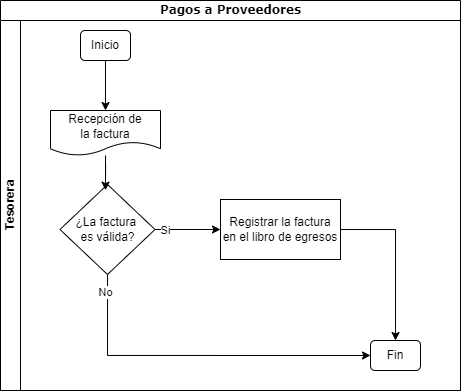
\includegraphics[width=1\textwidth]{resources/images/Diagrama de flujo de proceso pagos a proveedores-actual}
            \caption{Diagrama de flujo de procesos actual del pago de obligaciones financieras.}
            \label{fig:flujo-proceso-actual-pagos-proveedores}
        \end{figure}
        \item Multas
        \begin{enumerate}
            \item Se registra la multa en el libro de multas.
            \item Se guardan mediante fotos en los teléfonos de los directivos las infracciones cometidas por los propietarios o inquilinos.
            \item Se le notifica al propietario o inquilino la multa.
            \item El propietario o inquilino envía el comprobante de pago de la multa.
            \item La tesorera verifica el comprobante de pago.
            \begin{itemize}
                \item Si el comprobante es válido se procede al siguiente proceso.
                \item Si el comprobante no es válido se mantiene la multa y se finaliza el proceso.
            \end{itemize}
            \item Se registra el pago de la multa en el libro de ingresos.
            \item Se genera una orden de pago.
            \item La tesorera entrega la orden de pago a guardianía para que se le entregue al propietario o inquilino.
        \end{enumerate}
        \begin{figure}[H]
            \centering
            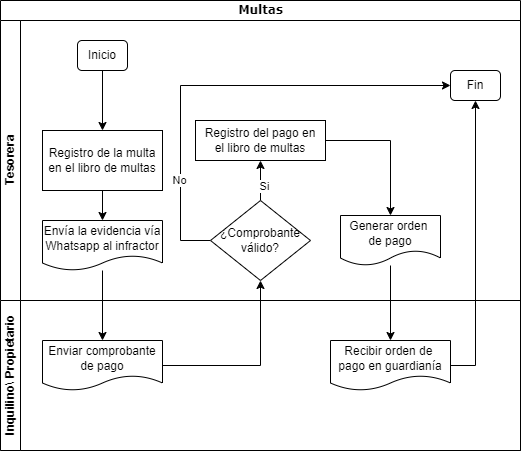
\includegraphics[width=1\textwidth]{resources/images/Diagrama de flujo de proceso multas actual}
            \caption{Diagrama de flujo de procesos actual de multas.}
            \label{fig:flujo-proceso-actual-multas}
        \end{figure}
    \end{enumerate}
\end{itemize}


\section{Desarrollo de la propuesta}\label{sec:desarrollo-propuesta}

Para el desarrollo de la propuesta se aplicó la metodología RAD la cual según\cite{bonilla_cadena_desarrollo_2022}, la autora menciona que esta metodología ayuda al desarrollo rápido de aplicaciones de una manera rápida y económica enfocada principalmente a empresas con baja disponibilidad de recursos y tiempo.

La metodología RAD se basa en cuatro fases principales:

\begin{itemize}
    \item Planificación de requerimientos \\
    En esta primera fase se identifican los requerimientos del sistema para satisfacer las necesidades del cliente y se establece el alcance del proyecto.
    \item Diseño de usuario\\
    Una vez identificados los requerimientos se crean modelos de diseño previos a la construcción del sistema los cuales son presentados a los usuarios para recibir retroalimentación.
    \item Construcción\\
    En esta fase se construye el sistema de acuerdo a los modelos de diseño previamente aprobados, mediante la codificación y pruebas del sistema.
    \item Transición
    La fase final en la que se realiza la entrega del sistema levantado en un entorno de producción real en donde se realizarán pruebas finales y se capacitará a los usuarios finales.
\end{itemize}

\subsection{Planificación de requerimientos} \label{subsec:planificacion-requerimientos}

En esta primera etapa se realizó un análisis de la información recopilada en las entrevistas, encuestas y en la situación actual descrita anteriormente.

En las siguientes tablas continuación se detallan en los usuarios identificados en la interacción con el sistema web y la aplicación móvil.
En la Tabla \ref{tab:table_requerimientos} se detallan los requerimientos del proyecto identificados por usuarios.

\begin{table}[H]
    \centering
    \caption{Descripción de los usuarios identificados en la interacción con el sistema web administrativo}
    \renewcommand*{\arraystretch}{1.4}
    \begin{longtable}{|p{0.2\textwidth}|p{0.7\textwidth}|}
        \hline
        \textbf{Usuario} & \textbf{Descripción}                                                                           \\
        \hline
        Administrador    & Usuario encargado de la administración de usuarios y la configuración de la geolocalización.   \\
        \hline
        Presidente       & Usuario encargado de la administración de parqueaderos, residencias, guardianía, convocatorias \\
        \hline
        Vicepresidente   & Usuario encargado de la administración de residencias, guardianía y convocatorias              \\
        \hline
        Tesorero         & Usuario encargado de la administración de los ingresos, multas y egresos                       \\
        \hline
        Secretario       & Usuario encargado de la administración de los eventos sociales y convocatorias                 \\
        \hline
    \end{longtable}\label{tab:table_usuarios_web}
\end{table}

\begin{table}[H]
    \centering
    \caption{Descripción de los usuarios identificados en la interacción con la aplicación móvil}
    \renewcommand*{\arraystretch}{1.4}
    \begin{longtable}{|p{0.2\textwidth}|p{0.7\textwidth}|}
        \hline
        \textbf{Usuario} & \textbf{Descripción}                                                                                                                                                 \\
        \hline
        Propietario      & Usuario encargado de registrar la asistencia en asambleas y votación, visualización de las obligaciones financieras relacionadas con su residencia o sus residencias \\
        \hline
        Inquilino        & Usuario encargado de registrar la asistencia en asambleas y visualización de las obligaciones financieras relacionadas con su residencia o sus residencias           \\
        \hline
    \end{longtable}\label{tab:table_usuarios_movil}
\end{table}

\begin{spacing}{1}

    \begin{center}
        \renewcommand*{\arraystretch}{1.4}
        \begin{longtable}[l]{|p{0.045\textwidth}|p{0.19\textwidth}|p{0.4\textwidth}|p{0.13\textwidth}| p{0.09\textwidth}|}
            \caption{Identificación de los requerimientos del sistema} \\
            \hline
            \textbf{ID} & \textbf{Requerimiento}                            & \textbf{Descripción}                                                                                                                                                                                                                                                                                                                                                                                                                                                                   & \textbf{Prioridad}         & \textbf{Riesgo}           \\
            \hline
            \multicolumn{5}{|l|}{ \textbf{Todos los usuarios} } \\
            \hline
            R1          & Iniciar sesión                                    & El usuario podrá iniciar sesión mediante su autenticación ingresando sus credenciales: cédula y contraseña & \multicolumn{1}{c|}{Alta} & \multicolumn{1}{c|}{Alto}\\
            \hline
            R2          & Cerrar sesión                                     & El usuario podrá finalizar la sesión en cualquier momento                                                                                                                                                                                                                                                                                                                                                                                                                              & \multicolumn{1}{c|}{Alta} & \multicolumn{1}{c|}{Bajo}\\
            \hline
            R3          & Recuperar contraseña                              & El usuario en caso de olvidar la contraseña podrá solicitar una contraseña nueva autogenerada por el sistema y enviada a su correo electrónico & \multicolumn{1}{c|}{Media} & \multicolumn{1}{c|}{Bajo}\\
            \hline
            R4          & Cambiar contraseña                                & El usuario podrá cambiar su contraseña en cualquier momento & \multicolumn{1}{c|}{Media} & \multicolumn{1}{c|}{Bajo}\\
            \hline
            \multicolumn{5}{|l|}{ \textbf{Administrador} } \\
            \hline
            R5          & Gestionar usuarios                                & El administrador podrá visualizar, registrar, inhabilitar o editar la información y roles de los demás usuarios  & \multicolumn{1}{c|}{Alta} & \multicolumn{1}{c|}{Alto}\\
            \hline
            R6          & Gestionar roles                                   & El administrador podrá visualizar o editar la descripción de los roles existentes en el sistema  & \multicolumn{1}{c|}{Media} & \multicolumn{1}{c|}{Bajo}\\
            \hline
            R7          & Gestionar pasajes                                 & El administrador podrá visualizar o editar la descripción de los pasajes existentes en el sistema  & \multicolumn{1}{c|}{Media} & \multicolumn{1}{c|}{Bajo}\\
            \hline
            R8          & Gestionar geolocalización                         & El administrador podrá editar la ubicación de las coordenadas y el radio de aceptación mediante la visualización de un mapa del lugar en donde se darán lugar las asambleas  & \multicolumn{1}{c|}{Alta} & \multicolumn{1}{c|}{Alto}\\
            \hline
            \multicolumn{5}{|l|}{ \textbf{Presidente} } \\
            \hline
            R9 & Gestionar estacionamientos & El presidente podrá visualizar, eliminar o actualizar la residencia asociada a cada parqueadero.
            También podrá visualizar o editar la descripción de los tipos de parqueaderos existentes & \multicolumn{1}{c|}{Alta} & \multicolumn{1}{c|}{Alto}\\
            \hline
            \multicolumn{5}{|l|}{ \textbf{Presidente y Vicepresidente} } \\
            \hline
            R10         & Gestionar residencias                             & El presidente o vicepresidente podrán visualizar, eliminar o actualizar el inquilino o propietario de cada residencia del conjunto & \multicolumn{1}{c|}{Alta} & \multicolumn{1}{c|}{Alto}\\
            \hline
            R11         & Gestionar guardias                                & El presidente o vicepresidente podrán visualizar, registrar, editar, o inhabilitar a los guardias de seguridad  & \multicolumn{1}{c|}{Alta} & \multicolumn{1}{c|}{Alto}\\
            \hline
            R12 & Gestionar actividades de guardianía & El presidente o vicepresidente podrá visualizar, registrar, editar, o eliminar las actividades de guardianía.
            También podrá cambiar el estado de cada actividad & \multicolumn{1}{c|}{Alta} & \multicolumn{1}{c|}{Alto}\\
            \hline
            R13         & Gestionar los tipos de incidentes                 & El presidente o vicepresidente podrán visualizar, registrar, editar, o inhabilitar los tipos de incidentes & \multicolumn{1}{c|}{Alta} & \multicolumn{1}{c|}{Alto}\\
            \hline
            R14         & Gestionar incidentes                              & El presidente o vicepresidente podrán visualizar, crear, editar, o eliminar los incidentes reportados por los guardías, asi como el cambio del estado del incidente & \multicolumn{1}{c|}{Alta} & \multicolumn{1}{c|}{Alto}\\
            \hline
            R15         & Gestionar convocatorias                           & El presidente o vicepresidente podrá visualizar, descargar, registrar, editar, finalizar o eliminar las convocatorias,  & \multicolumn{1}{c|}{Alta} & \multicolumn{1}{c|}{Alto}\\
            \hline
            R16         & Gestionar asistencias de las asambleas            & Las convocatorias de tipo asamblea son las únicas que poseerán registro de asistencias, de tal manera que el presidente o vicepresidente podrán realizar el registro manual de las asistencias, asi como descargar un reporte de inasistentes & \multicolumn{1}{c|}{Alta} & \multicolumn{1}{c|}{Alto}\\
            \hline
            R17         & Gestionar votaciones de las asambleas             & Las convocatorias de tipo asamblea son las únicas que poseerán votaciones, de tal manera que el presidente o vicepresidente podrán visualizar, editar, habilitar el voto o eliminar de cada pregunta propuesta a votación, asi como también poder visualizar la información de votación de cada votante & \multicolumn{1}{c|}{Alta} & \multicolumn{1}{c|}{Alto}\\
            \hline
            \multicolumn{5}{|l|}{ \textbf{Tesorero} } \\
            \hline
            R18         & Gestionar ingresos mensuales                      & Posterior a la entrega física o digital del comprobante de pago por parte del residente la tesorera procede a registrar los datos del pago junto con el comprobante teniendo en cuenta el último mes de pago y hasta que mes está abonando el residente y posteriormente se envía al correo electrónico un respaldo del registro del pago, adicional a esto también puede visualizar, editar la información así como actualizar el comprobante de pago o eliminar el registro del pago & \multicolumn{1}{c|}{Alta} & \multicolumn{1}{c|}{Alto}\\
            \hline
            R19         & Gestionar ingresos casuales                       & Posterior a la entrega física o digital del comprobante de pago por parte del residente la tesorera procede a registrar los datos del pago junto con el comprobante y posteriormente se envía al correo electrónico un respaldo del registro del pago, adicional a esto también puede visualizar, editar la información así como actualizar el comprobante de pago o eliminar el registro del pago & \multicolumn{1}{c|}{Alta} & \multicolumn{1}{c|}{Alto}\\
            \hline
            R20 & Gestionar multas & La tesorera podrá visualizar, crear, editar o eliminar las multas.
            Los residentes deben presentar de manera física o digital el comprobante del pago de la multa por el monto indicado y posterior a su revisión se procede a subir el comprobante y a actualizar el estado del pago de la multa, posteriormente se envía al correo electrónico un respaldo del registro del pago & \multicolumn{1}{c|}{Alta}  & \multicolumn{1}{c|}{Alto}\\
            \hline
            \multicolumn{5}{|l|}{ \textbf{Secretario} } \\
            \hline
            R21         & Gestionar eventos sociales                        & El secretario podrá visualizar, registrar, editar, o eliminar los eventos sociales. & \multicolumn{1}{c|}{Media} & \multicolumn{1}{c|}{Bajo}\\
            \hline
            R22         & Subir actas                           & El secretario podrá subir actas de las convocatorias & \multicolumn{1}{c|}{Media} & \multicolumn{1}{c|}{Bajo}\\
            \hline
            \multicolumn{5}{|l|}{ \textbf{Propietario e Inquilino} } \\
            \hline
            R23         & Visualizar el calendario                          & El propietario o inquilino podrán visualizar el calendario de eventos sociales y asambleas próximas & \multicolumn{1}{c|}{Media} & \multicolumn{1}{c|}{Bajo}\\
            \hline
            R24         & Visualizar estado de las obligaciones financieras & El propietario o inquilino podrán visualizar el estado financiero de sus obligaciones financieras de todas sus residencias o parqueaderos & \multicolumn{1}{c|}{Media} & \multicolumn{1}{c|}{Bajo}\\
            \hline
            R25         & Visualizar asamblea del día                       & El propietario o inquilino podrán visualizar la asamblea únicamente si se da en ese día & \multicolumn{1}{c|}{Alta} & \multicolumn{1}{c|}{Bajo}\\
            \hline
            R26         & Registrar asistencia                              & El propietario o inquilino podrán registrar su asistencia siempre que se encuentre dentro del rango de geolocalización registrado por el administrador del sistema & \multicolumn{1}{c|}{Alta} & \multicolumn{1}{c|}{Alto}\\
            \hline
            \multicolumn{5}{|l|}{ \textbf{Propietario} } \\
            \hline
            R27         & Registrar voto                                    & El propietario podrá registrar su voto en las preguntas que se encuentren habilitadas para su voto siempre que se encuentre dentro del rango de geolocalización registrado por el administrador del sistema y tenga registrada la asistencia& \multicolumn{1}{c|}{Alta} & \multicolumn{1}{c|}{Alto}\\
            \hline
        \end{longtable}\label{tab:table_requerimientos}
    \end{center}
\end{spacing}

Una vez definidos los requerimientos del sistema se define el plan de trabajo en cada iteración para el desarrollo de los sistemas.

\begin{spacing}{1}
    \begin{center}
        \renewcommand*{\arraystretch}{1.4}
        \begin{longtable}[l]{|p{0.17\textwidth}|p{0.045\textwidth}|p{0.055\textwidth}|p{0.37\textwidth}| p{0.09\textwidth}|p{0.09\textwidth}| }
            \caption{Identificación de los requerimientos del sistema} \\
            \hline
            \multirow{2}{*}{\textbf{N° Iteración}} & \multirow{2}{*}{\textbf{N°}} & \multirow{2}{*}{\textbf{ID}} & \multirow{2}{*}{\textbf{Requerimiento}} & \multicolumn{2}{c|}{\textbf{Tiempo estimado}}\\
            \cline{5-6}
            & & & & \textbf{Horas} & \textbf{dias} \\
            \hline
            \multirow{8}{*}{Iteración 1} & 1 & R1 & Iniciar sesión & 6 & 1 \\
            \cline{2-6}
             & 2 & R2 & Cerrar sesión & 1 & 1 \\
            \cline{2-6}
             & 3 & R3 & Recuperar contraseña & 2 & 1 \\
            \cline{2-6}
             & 4 & R4 & Cambiar contraseña & 1 & 1 \\
            \cline{2-6}
             & 5 & R5 & Gestionar usuarios & 10 & 2 \\
            \cline{2-6}
             & 6 & R6 & Gestionar roles & 3 & 1 \\
            \cline{2-6}
             & 7 & R7 & Gestionar pasajes & 3 & 1 \\
            \cline{2-6}
             & 8 & R8 & Gestionar geolocalización & 6 & 1 \\
            \hline
            \multirow{9}{*}{Iteración 2} & 9 & R9 & Gestionar estacionamientos & 16 & 2 \\
            \cline{2-6}
             & 10 & R10 & Gestionar residencias & 8 & 1 \\
            \cline{2-6}
             & 11 & R11 & Gestionar guardias & 6 & 1 \\
            \cline{2-6}
             & 12 & R12 & Gestionar actividades de guardianía & 8 & 1 \\
            \cline{2-6}
             & 13 & R13 & Gestionar los tipos de incidentes & 4 & 1 \\
            \hline
             & 14 & R14 & Gestionar incidentes & 8 & 1 \\
            \cline{2-6}
             & 15 & R15 & Gestionar convocatorias & 16 & 2 \\
            \cline{2-6}
             & 16 & R16 & Gestionar asistencias de las asambleas & 8 & 1 \\
            \cline{2-6}
             & 17 & R17 & Gestionar votaciones de las asambleas & 10 & 2 \\
            \hline
            \multirow{10}{*}{Iteración 3} & 18 & R18 & Gestionar ingresos mensuales & 16 & 2 \\
            \cline{2-6}
             & 19 & R19 & Gestionar ingresos casuales & 8 & 1 \\
            \cline{2-6}
             & 20 & R20 & Gestionar multas & 14 & 2 \\
            \cline{2-6}
             & 21 & R21 & Gestionar eventos sociales & 8 & 1 \\
            \cline{2-6}
             & 22 & R22 & Subir actas & 2 & 1 \\
            \cline{2-6}
             & 23 & R23 & Visualizar el calendario & 4 & 1 \\
            \cline{2-6}
             & 24 & R24 & Visualizar estado de las obligaciones financieras & 12 & 2 \\
            \cline{2-6}
             & 25 & R25 & Visualizar asamblea del día & 4 & 1 \\
            \cline{2-6}
             & 26 & R26 & Registrar asistencia & 8 & 1 \\
            \cline{2-6}
             & 27 & R27 & Registrar voto & 8 & 1 \\
            \hline
        \end{longtable}
    \end{center}
\end{spacing}

\subsection{Diseño de usuario} \label{subsec:diseno-usuario}
\subsubsection{Análisis de los procesos sistematizados propuestos}

A continuación se detallaran los procesos sistematizados para la administración de parqueaderos, convocatorias y administración financiera.

\begin{itemize}
    \item Proceso de administración de parqueaderos (Zona azul).
    \begin{enumerate}
        \item Se verifica que el propietario o inquilino este registrado en el sistema.
        \begin{enumerate}
            \item Si está registrado se procede al siguiente proceso.
            \item Si no está registrado se le notifica al administrador para su registro en el sistema y se repite el proceso.
        \end{enumerate}
        \item El presidente solicita enviar la documentación requerida para la asignación de un parqueadero.
        \begin{enumerate}
            \item Si entrega la documentación completa se procede al siguiente proceso.
            \item Si no entrega la documentación completa se finaliza el proceso.
        \end{enumerate}
        \item El presidente muestra en el sistema el mapa de parqueaderos disponibles.
        \item El propietario o inquilino debe abonar diez dólares por la asignación del parqueadero y enviar el comprobante de pago a la tesorera.
        \item La tesorera verifica el comprobante de pago de diez dólares por la asignación del parqueadero.
        \item Se registra el pago en los ingresos mensuales en el sistema.
        \item Se sube el comprobante de pago al sistema.
        \item Se envía por correo electrónico el respaldo de pago al propietario o inquilino.
        \item El presidente asigna el parqueadero al domicilio relacionado al propietario o inquilino.
        \item El sistema genera una carta de compromiso.
    \end{enumerate}

    \item Proceso de administración de convocatorias.
    \begin{enumerate}
        \item La directiva del conjunto se reúne para definir la fecha de la convocatoria.
        \item Se registra en el sistema la convocatoria y se notifica a los propietarios o inquilinos mediante la aplicación móvil.
        \item Se lleva a cabo la convocatoria.
        \begin{itemize}
            \item Si es una asamblea se procede al siguiente proceso.
            \item Si es una reunión o sesión de directiva se salta al proceso 6.
        \end{itemize}
        \item Los inquilinos o propietarios registran su asistencia en la aplicación móvil.
        \begin{enumerate}
            \item Si no esta registrado en el sistema el presidente o vicepresidente registra su asistencia de su domicilio al que representa.
            \item Si esta registrado en el sistema se procede al siguiente proceso.
        \end{enumerate}
        \item Se verifica la ubicación del propietario o inquilino mediante la geolocalización.
        \begin{itemize}
            \item Si se encuentra en el rango de geolocalización se registra la asistencia y se procede al siguiente proceso.
            \item Si no se encuentra en el rango de geolocalización no se registra la asistencia.
        \end{itemize}
        \item Se tratan los temas de la convocatoria.
        \item Se propone una votación de los temas a tratar.
        \begin{itemize}
            \item Si existe una votación se procede al siguiente proceso.
            \item Si no existe una votación se salta al proceso 14.
        \end{itemize}
        \item Se registra la votación en el sistema.
        \item Se habilita el voto a los propietarios o inquilinos.
        \item El sistema verifica que el usuario que va a votar sea propietario.
        \begin{itemize}
            \item Si es propietario se procede al siguiente proceso.
            \item Si no es propietario no se registra el voto.
        \end{itemize}
        \item Los propietarios registran su voto en la aplicación móvil.
        \item Se verifica la ubicación del propietario mediante la geolocalización.
        \begin{itemize}
            \item Si se encuentra en el rango de geolocalización se registra el voto y se procede al siguiente proceso.
            \item Si no se encuentra en el rango de geolocalización no se registra el voto.
        \end{itemize}
        \item Se muestra el resultado de la votación desde el sistema.
        \item Se finaliza la convocatoria.
        \item Se sube el acta de la convocatoria al sistema.
        \begin{itemize}
            \item Si es una asamblea se procede al siguiente proceso.
            \item Si es una reunión o sesión de directiva se finaliza el proceso.
        \end{itemize}
        \item Se genera el informe de inasistencia de los propietarios o inquilinos desde el sistema.
        \item Se envía el informe de asistencia a los residentes y se registra la respectiva multa en el sistema.
        \item El propietario o inquilino puede presentar una justificación por la inasistencia en las siguientes 24 horas.
        \item Se verifica la justificación presentada.
        \begin{itemize}
            \item Si la justificación es válida se procede a eliminar la multa del sistema y se finaliza el proceso.
            \item Si la justificación no es válida la multa se mantiene y termina el proceso.
        \end{itemize}
    \end{enumerate}


    \item Proceso de administración financiera.
    \begin{enumerate}
        \item Pagos de obligaciones financieras mensuales
        \begin{enumerate}
            \item El inquilino realiza el pago de la mensualidad de sus obligaciones financieras.
            \item El inquilino envía el comprobante de pago a la tesorera.
            \item La tesorera verifica el comprobante de pago.
            \begin{itemize}
                \item Si el comprobante es válido se procede al siguiente proceso.
                \item Si el comprobante no es válido se finaliza el proceso.
            \end{itemize}
            \item La tesorera selecciona la residencia del inquilino o propietario.
            \item El sistema verifica hasta que mes abonó el inquilino en su anterior pago.
            \begin{itemize}
                \item Si el inquilino tiene abonos anteriores el sistema coloca el mes siguiente de manera automática y se procede al siguiente paso.
                \item Si el inquilino no tiene abonos se procede al siguiente paso.
            \end{itemize}
            \item Se registra el pago en el sistema.
            \item Se sube el comprobante de pago al sistema.
            \item Se genera una orden de pago.
            \item Se envía por correo electrónico el respaldo de pago al inquilino o propietario.
        \end{enumerate}

        \item Pagos a proveedores
        \begin{enumerate}
            \item El proveedor envía la factura a la tesorera.
            \item La tesorera verifica la factura.
            \begin{itemize}
                \item Si la factura es válida se procede al siguiente proceso.
                \item Si la factura no es válida se finaliza el proceso.
            \end{itemize}
            \item La tesorera verifíca si el proveedor está registrado en el sistema.
            \begin{itemize}
                \item Si el proveedor está registrado se procede al siguiente proceso.
                \item Si el proveedor no está registrado se le registra en el sistema y se repite el proceso.
            \end{itemize}
            \item La tesorera registra la factura en el sistema.
            \item Se sube la factura al sistema.
        \end{enumerate}

        \item Multas
        \begin{enumerate}
            \item Se registra la multa en el sistema.
            \item Se suben evidencias de la multa al sistema.
            \item Se le notifica al propietario o inquilino la multa mediante la aplicación móvil.
            \item El propietario o inquilino envía el comprobante de pago de la multa.
            \item La tesorera verifica el comprobante de pago.
            \begin{itemize}
                \item Si el comprobante es válido se procede al siguiente proceso.
                \item Si el comprobante no es válido se mantiene la multa y se finaliza el proceso.
            \end{itemize}
            \item Se actualiza el estado de la multa en el sistema.
            \item Se genera una orden de pago.
            \item El sistema envía por correo electrónico el respaldo de pago al propietario o inquilino.
        \end{enumerate}

    \end{enumerate}
\end{itemize}



\chapter{CONCLUSIONES Y RECOMENDACIONES}\label{ch:conclusiones-y-recomendaciones}
\section{Conclusiones}

El presente trabajo de titulación se desarrolló con el objetivo de proponer una solución tecnológica que permita mejorar la gestión de la administración del Conjunto habitacional  {\textquotedblleft}El Portal de la Viña{\textquotedblright}, a través de la implementación de un sistema web y móvil que permita a la directiva y a los residentes gestionar de una manera más ágil y cómoda los procesos administrativos, así como proporcionar un acceso más rápido a la información del conjunto habitacional.

\begin{itemize}
    \item Con la ayuda de las entrevistas y encuestas se pudo identificar los problemas principales que enfrentaba la directiva del conjunto habitacional, con lo cual se logró proponer una solución tecnológica que permita mejorar la gestión y el acceso a la información.
    La entrevista con el presidente de la directiva fue en mayor parte la que permitió identificar los problemas administrativos, tales como la deficiencia en la toma de asistencia en las asambleas, la dificultad de acceder a la información de las obligaciones financieras de los residentes y la mala organización de la información de los parqueaderos.
    Con estos problemas analizados se pudo evidenciar la necesidad de tener un sistema que permita gestionar de manera eficiente la información del conjunto habitacional.
    \item El uso de frameworks de desarrollo ha demostrado que son herramientas que permiten acelerar el proceso de desarrollo de software, ya que proveen de un marco de trabajo ya definido con el cual se puede agilizar de forma considerable el desarrollo de cualquier software, además de que existe una gran cantidad de documentación y una comunidad activa que puede ayudar a resolver problemas que se presenten durante el desarrollo.
    Sin embargo, la elección del framework adecuado dependerá de las necesidades del proyecto y de la experiencia de las personas involucradas en el desarrollo.

    \item La metodología de desarrollo de software debe ser seleccionada de acuerdo a la naturaleza del proyecto, ya que depende directamente de los requerimientos y del equipo de trabajo.
    En el caso partícular de este proyecto se pudo observar que el uso de una metodología ágil como RAD permitió tener un desarrollo rápido y con la participación activa de los usuarios, lo cual permitió tener un producto final que cumplió con las necesidades y expectativas del cliente.
    \item La implementación de las validaciones mediante el uso de la geolocalización junto con el cálculo de la distancia de Haversiné demostraron ser unas herramientas útiles para verificar la ubicación de los residentes durante las asambleas.
    Esta estrategia ha tenido un impacto positivo en la confiabilidad del proceso de asistencias y votaciones, previniendo el mal uso de la aplicación y garantizando la autenticidad de los datos durante las sesiones de asamblea.
\end{itemize}
\section{Recomendaciones}\label{sec:recomendaciones}
\begin{itemize}
    \item Se recomienda que la directiva del conjunto habitacional {\textquotedblleft}El Portal de la Viña{\textquotedblright} realice una capacitación a los residentes sobre el uso de la aplicación móvil y web, con el fin de que puedan aprovechar al máximo las funcionalidades que ofrece el sistema.
    \item Se sugiere llevar a cabo una concientización a los residentes por parte de la directiva, para que se utilicen las herramientas tecnológicas de manera responsable, ya que el uso innecesario puede conllevar a un incremento de costos en los servicios implementados de AWS.
    \item Dada la importancía de la información que se maneja en el sistema, se recomienda realizar respaldos de manera periódica de la base de datos, con el fin de evitar la pérdida de información en caso de que ocurra algún fallo en el sistema.
    \item En consideración de la información que se maneja en el sistema, se sugiere una integración con el sistema actual de control de tarjetas de acceso, con el fin de tener centralizada toda la información y evitar el uso de múltiples sistemas.
    \newpage
    \item AWS provee una gran cantidad de servicios por lo cual se recomienda tener un conocimiento mínimo a cerca de esta plataforma, ya que el uso de servicios innecesarios puede conllevar a una mayor inversion de recursos y, por lo tanto, a un incremento en los costos.
\end{itemize}

%C. Materiales de referencia
\bibliographystyle{biblio/IEEEtran}
\bibliography{biblio/main}
\addcontentsline{toc}{chapter}{\bfseries REFERENCIAS BIBLIOGRÁFICAS}

\chapter*{Anexos}
\addcontentsline{toc}{chapter}{\bfseries\uppercase{Anexos}}

% \addtocontents{toc}{\protect\setcounter{tocdepth}{0}}
\appendix

\renewcommand{\thetable}{\theappendixs\arabic{table}}
\renewcommand{\thefigure}{\theappendixs\arabic{figure}}
\renewcommand{\thelstlisting}{\theappendixs\arabic{lstlisting}}
\captionsetup{list=no}

\appendixs{Guía de entrevista a la directiva del conjunto habitacional {\textquotedblleft}El Portal de la Viña{\textquotedblright}}
\label{app:guia-entrevista-directiva}
\begin{table}[H]
	\caption{Guía de entrevista a la directiva del conjunto habitacional {\textquotedblleft}El Portal de la Viña{\textquotedblright}}
	\label{tab:guia-entrevista-directiva}


	\begin{center}
		\begin{footnotesize}
		\begin{tabular}[c]{|p {0.03\textwidth}|p{0.6\textwidth}|p{0.15\textwidth}|p{0.15\textwidth}|}
			\hline
			\multicolumn{1}{|c|}{\textbf{N.}} & \multicolumn{1}{c|}{\textbf{Pregunta}} & \multicolumn{1}{c|}{\textbf{Respuesta}} & \multicolumn{1}{c|}{\textbf{Observación}} \\
			\hline
			1 & ¿Cuáles son sus funciones administrativas o financieras como parte de la directiva? & & \\ \hline
			2 & ¿Cómo miembro de la directiva tiene alguna función extra que la realice de forma extraordinaria como parte de su iniciativa? & &\\ \hline
			3 & ¿Qué reportes, documentos o certificados entrega como parte de directiva y con qué información? & &\\ \hline
			4 & ¿Cuál es el proceso actual para la adquisición de un parqueadero tanto particular como de zona azul y en el caso de requerir alguna información o documento, existe la posibilidad de poder entregar alguno de manera digital? & &\\ \hline
			5 & ¿De que manera se lleva el registro de los parqueaderos? & &\\ \hline
			6 & ¿Cuáles es el proceso actual para la adquisición de servicios de proveedores (guardianía, internet, jardinería, etc.)? & &\\ \hline
			7 & ¿De qué manera se lleva la contabilidad del conjunto habitacional y que reportes se suelen presentar y con qué información? & &\\ \hline
			8 & ¿De que manera se comunica a los residentes del condominio eventos sociales o convocatorias de asambleas? & &\\ \hline
			9 & ¿Cuál es el proceso actual para el registro de asistencia y las votaciones en las asambleas? & &\\ \hline
			10 & ¿Cuándo una residente falta a una reunión de asamblea que penalizaciones o multas recibe? & &\\ \hline
			11 & ¿Qué problemas o inconvenientes han tenido con los procesos administrativos o financieros actuales? & &\\ \hline
			12 & ¿Actualmente cómo funciona el buzón de quejas/sugerencias? & &\\ \hline
			13 & ¿Dónde manejan la información de los pagos (multas, alícuotas, parqueaderos, etc.), asambleas, eventos sociales, pagos a proveedores y demás información importante? & &\\
			\hline
		\end{tabular}
		\end{footnotesize}
	\end{center}

\end{table}

\newpage
\appendixs{Encuesta de necesidades a los residentes del conjunto habitacional {\textquotedblleft}El Portal de la Viña{\textquotedblright}}
\label{app:encuesta-residentes}

\begin{center}
	\begin{small}
		\begin{longtable}[c]{|p{0.6\textwidth}|p{0.35\textwidth}|}
			\caption{Encuesta de necesidades a los residentes del conjunto habitacional {\textquotedblleft}El Portal de la Viña{\textquotedblright}} \\
			\hline
			\textbf{Pregunta} & \textbf{Respuesta} \\
			\hline
			¿Cree usted que el proceso actual para obtener la información de las obligaciones financieras (pagos, multas, etc.) de su domicilio es eficiente? &
			\begin{itemize}
				\item Totalmente de acuerdo
				\item De acuerdo
				\item Ni de acuerdo ni en desacuerdo
				\item En desacuerdo
				\item Totalmente en desacuerdo
			\end{itemize} \\
			\hline
			¿Con que frecuencia solicita la información de las obligaciones financieras (pagos, multas, etc.) de su domicilio a tesorería? &
			\begin{itemize}
				\item Por lo menos una vez al mes
				\item Dos veces al mes
				\item Tres veces al mes
				\item Cuatro veces al mes
				\item Más de cuatro veces al mes
			\end{itemize}\\
			\hline
			¿Cree usted que el proceso actual para el registro de asistencias durante la asamblea es eficiente en términos de tiempo? &
			\begin{itemize}
				\item Totalmente de acuerdo
				\item De acuerdo
				\item Ni de acuerdo ni en desacuerdo
				\item En desacuerdo
				\item Totalmente en desacuerdo
			\end{itemize} \\
			\hline
			¿Considera usted que el conteo actual de las votaciones durante las asambleas es transparente y eficiente? &
			\begin{itemize}
				\item Totalmente de acuerdo
				\item De acuerdo
				\item Ni de acuerdo ni en desacuerdo
				\item En desacuerdo
				\item Totalmente en desacuerdo
			\end{itemize} \\
			\hline
			¿Ha experimentado retrasos en la entrega de los comprobantes de pagos? &
			\begin{itemize}
				\item Si
				\item No
			\end{itemize} \\
			\hline
			¿Con que frecuencia olvida que el pago de alícuotas de su domicilio esta por vencer? &
			\begin{itemize}
				\item Muy frecuentemente
				\item Frecuentemente
				\item Ocasionalmente
				\item Raramente
				\item Nunca
			\end{itemize}\\
			\hline
			¿Con que frecuencia ha utilizado el buzón de quejas/sugerencias? &
			\begin{itemize}
				\item Nunca lo he usado
				\item Al menos una vez al mes
				\item Dos veces al mes
				\item Tres veces al mes
				\item Más de tres veces al mes
			\end{itemize} \\
			\hline
			¿Considera usted que los medios actuales (whatsapp/pizarrón en la garita) que utiliza la directiva para publicar comunicados son eficientes? &
			\begin{itemize}
				\item Totalmente de acuerdo
				\item De acuerdo
				\item Ni de acuerdo ni en desacuerdo
				\item En desacuerdo
				\item Totalmente en desacuerdo
			\end{itemize} \\
			\hline
			¿Preferiría utilizar una aplicación móvil que le permita revisar la información de las obligaciones financieras de su domicilio, el registro de su asistencia y voto durante las asambleas, se le envíen notificaciones recordándole los pagos por vencer o que ha sido multado por alguna infracción? &
			\begin{itemize}
				\item Si
				\item No
			\end{itemize} \\
			\hline
		\end{longtable}
	\end{small}
\end{center}

\newcolumntype{C}[1]{>{\centering\arraybackslash}m{#1}}
\appendixs{Encuesta TAM del sistema web administrativo}
\label{app:encuesta-tam}
\begin{center}
	\begin{small}
		\begin{table}[ht]
		\begin{center}
			\caption{Encuesta de aceptación TAM \#1}
			\bigbreak
			\begin{tabular}{ *{5}{C{2cm}} }
				\hline
				\multicolumn{5}{ c }{\textbf{ENCUESTA DE ACEPTACIÓN TAM SISTEMA WEB}} \\ \hline
				\multicolumn{5}{p{.7\textwidth}}{En una escala de Likert indique su grado de aceptación con las siguientes ponderaciones: } \\ \hline
				\centering 1             & 2             & 3       & 4          & 5                     \\ \hline
				Totalmente en desacuerdo & En desacuerdo & Neutral & De acuerdo & Totalmente de acuerdo \\ \hline
				\textbf{PU} & \multicolumn{4} {c}{\textbf{Utilidad Percibida}} \\ \hline
				PU1 & \multicolumn{4}{p{.7\textwidth}}{El sistema facilita las tareas de gestión del conjunto residencial} \\ \hline
				PU2 & \multicolumn{4}{p{.7\textwidth}}{Mejora la eficiencia en las operaciones diarias del conjunto residencial} \\ \hline
				PU3 & \multicolumn{4}{p{.7\textwidth}}{Proporciona información relevante para la toma de decisiones} \\ \hline
				PU4 & \multicolumn{4}{p{.7\textwidth}}{Mejora la calidad de vida/comodidad para los residentes} \\ \hline
				\textbf{PEOU} & \multicolumn{4}{ c }{\textbf{Facilidad de Uso Percibida}} \\ \hline
				PEOU1 & \multicolumn{4}{p{.7\textwidth}}{Es fácil aprender a utilizar el sistema de gestión residencial} \\ \hline
				PEOU2 & \multicolumn{4}{p{.7\textwidth}}{La navegación por el sistema es clara y lógica} \\ \hline
				PEOU3 & \multicolumn{4}{p{.7\textwidth}}{El diseño de la interfaz es intuitivo y amigable} \\ \hline
				PEOU4 & \multicolumn{4}{p{.7\textwidth}}{Es cómodo interactuar desde diferentes navegadores web} \\ \hline
			\end{tabular}
			\label{tab:tam_encuesta_web}
			\bigbreak
		\end{center}
	\end{table}
	\end{small}
\end{center}

\newpage
\newcolumntype{C}[1]{>{\centering\arraybackslash}m{#1}}
\appendixs{Encuesta TAM del sistema web administrativo}
\label{app:encuesta-tam-app}
\begin{center}
	\begin{small}
		\begin{table}[h]
			\begin{center}
				\caption{Encuesta de aceptación TAM \#2}
				\begin{tabular}{ *{5}{C{2cm}} }
					\hline
					\multicolumn{5}{ c }{\textbf{ENCUESTA DE ACEPTACIÓN TAM APLICACIÓN MÓVIL}} \\ \hline
					\multicolumn{5}{p{.7\textwidth}}{En una escala de Likert indique su grado de aceptación con las siguientes ponderaciones: } \\ \hline
					\centering 1             & 2             & 3       & 4          & 5                     \\ \hline
					Totalmente en desacuerdo & En desacuerdo & Neutral & De acuerdo & Totalmente de acuerdo \\ \hline
					\textbf{PU} & \multicolumn{4} {c}{\textbf{Utilidad Percibida}} \\ \hline
					PU1 & \multicolumn{4}{p{.7\textwidth}}{La aplicación ofrece información relevante sobre próximos eventos en el conjunto residencial} \\ \hline
					PU2 & \multicolumn{4}{p{.7\textwidth}}{Las notificaciones de pagos son claras y fáciles de comprender en la aplicación.} \\ \hline
					PU3 & \multicolumn{4}{p{.7\textwidth}}{La opción de votaciones dentro de la aplicación es útil y accesible.} \\ \hline
					PU4 & \multicolumn{4}{p{.7\textwidth}}{La aplicación mejora la interacción y la comunicación entre los residentes.} \\ \hline

					\textbf{PEOU} & \multicolumn{4}{ c }{\textbf{Facilidad de Uso Percibida}} \\ \hline
					PEOU1 & \multicolumn{4}{p{.7\textwidth}}{Es sencillo navegar por la aplicación para encontrar la información deseada.} \\ \hline
					PEOU2 & \multicolumn{4}{p{.7\textwidth}}{El diseño de la aplicación es intuitivo y fácil de comprender.} \\ \hline
					PEOU3 & \multicolumn{4}{p{.7\textwidth}}{La aplicación ofrece una experiencia cómoda al interactuar desde distintos dispositivos móviles.} \\ \hline
					PEOU4 & \multicolumn{4}{p{.7\textwidth}}{La función de votación en la aplicación es fácil de usar y comprender.} \\ \hline
				\end{tabular}
				\label{tab:tam_encuesta_app}
				\bigbreak
				Elaborado por: el investigador
			\end{center}
		\end{table}
	\end{small}
\end{center}

\newpage
\appendixs{Dependencias de la API} \label{app:dependencias-api}

\begin{figure}[H]
    \centering
    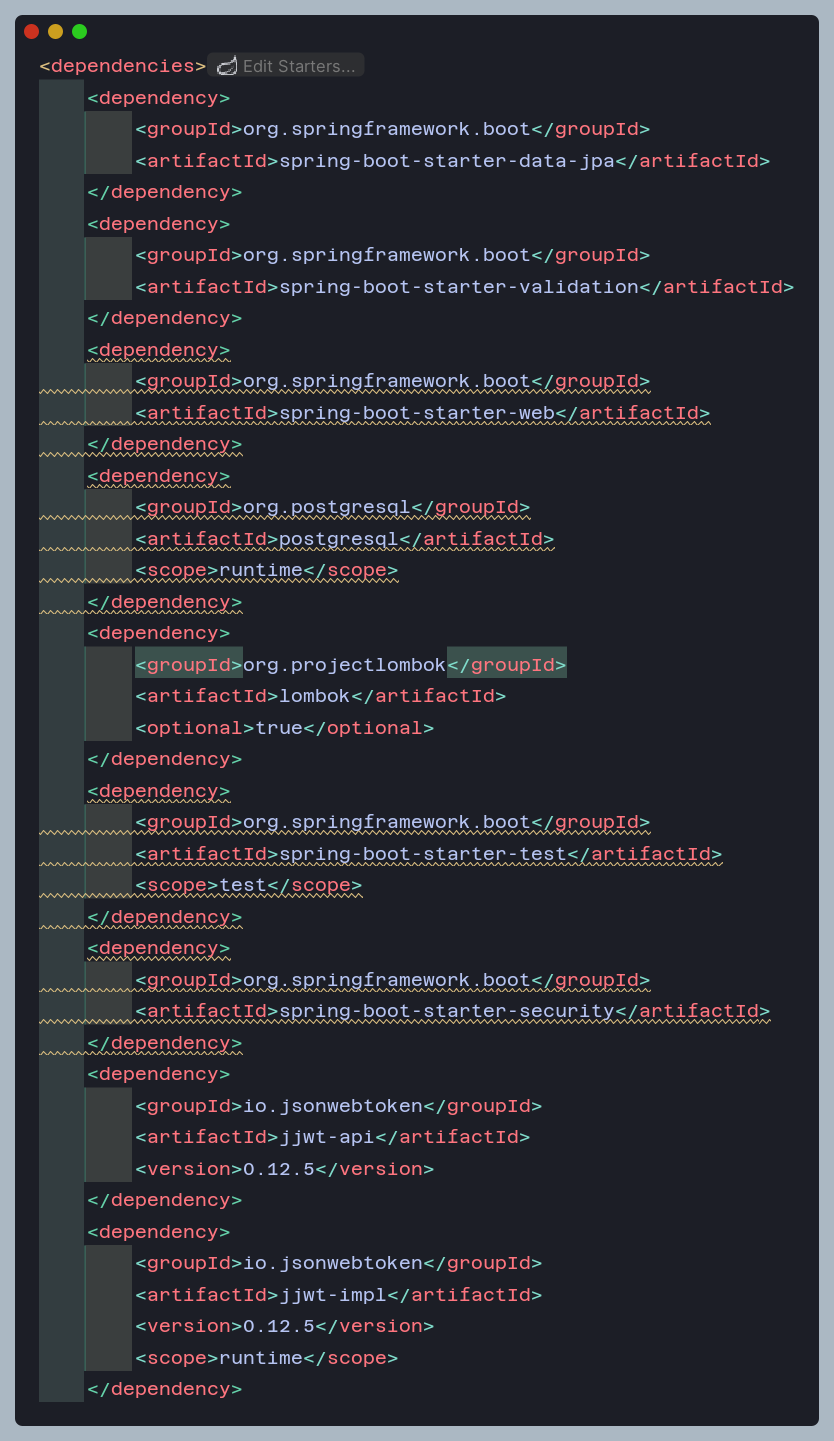
\includegraphics[width=.8\textwidth]{resources/images/dependencias-anexo-1}\label{fig:dependencias Api 1}
\end{figure}

\begin{figure}[H]
    \centering
    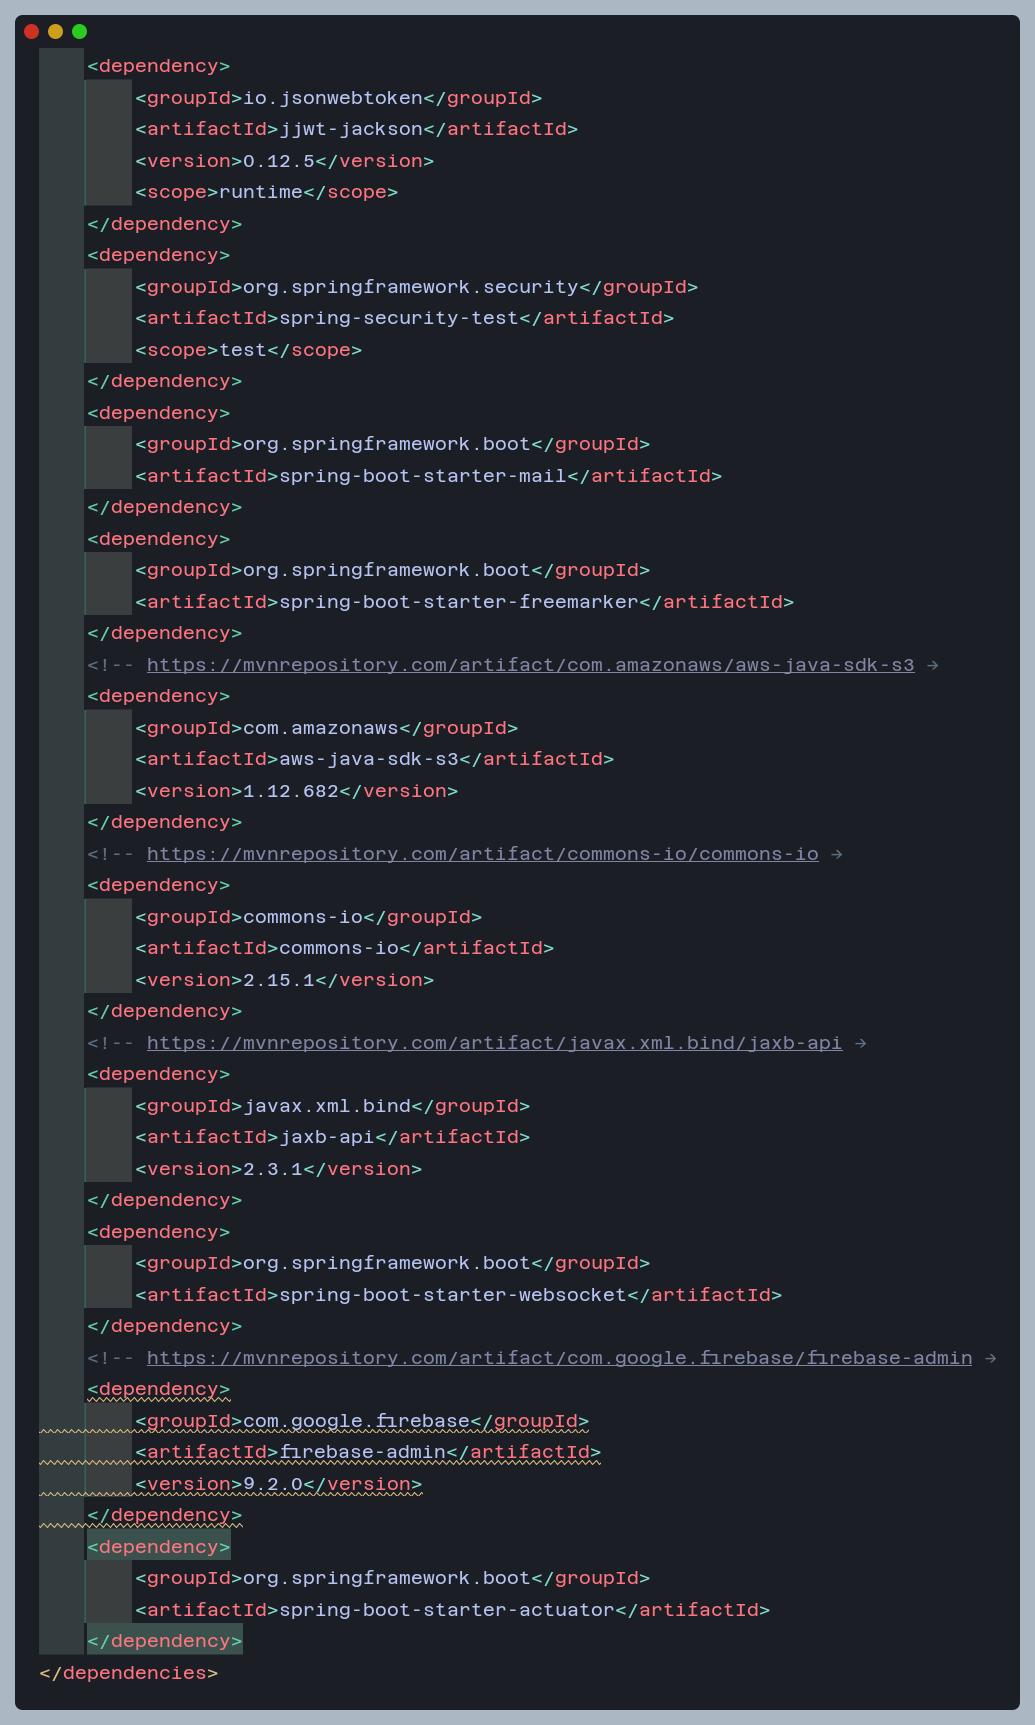
\includegraphics[width=.8\textwidth]{resources/images/dependencias-anexo-2}\label{fig:dependencias Api 2}
\end{figure}



\end{document}
